\documentclass[14pt,oneside]{extreport}
\usepackage[a4paper,right=3cm,top=2.5cm,left=2.5cm,bottom=2.5cm]{geometry}

\usepackage[nottoc]{tocbibind}
\usepackage{listings, subcaption}
\usepackage{amsmath, amsthm}
\usepackage{longtable}
\usepackage{graphicx}
\usepackage{algorithm}
%%%% BIB
%\usepackage[authoryear]{natbib}
\usepackage{amssymb}
\usepackage{pdflscape}
\usepackage{afterpage}

%\pagestyle{empty}
\usepackage{indentfirst}
\usepackage{geometry}

\usepackage{indentfirst}
\usepackage{geometry}
\geometry{
	a4paper,
	total={170mm,257mm},
	left=30mm,
	right=30mm,
	top=25mm,
	bottom=25mm
}
\usepackage{longtable}
\usepackage{makecell}
\usepackage{graphicx}
\usepackage{amssymb}
%\usepackage{enumitem}
\usepackage{amsmath, amsthm, amssymb, listings, multirow, wrapfig}
\usepackage{multirow, booktabs}

\usepackage{footnote}
\usepackage{amsmath,amsfonts,stmaryrd,amssymb} % Math packages
\usepackage{algorithm}
\usepackage{algorithmic}
\usepackage{mathtools}
\usepackage{commath}
\usepackage{verbatim}
\usepackage{enumerate} % Custom item numbers for enumerations
\usepackage{tikz}
\usepackage[colorlinks=true,citecolor=blue]{hyperref}%
\usetikzlibrary{arrows}


\usepackage[framemethod=tikz]{mdframed}

\usepackage{listings} % File listings, with syntax highlighting
\lstset{
	basicstyle=\ttfamily, % Typeset listings in monospace font
}

%%%% Renewdefs and Envs.
\graphicspath{{./Figures/}}

\newtheorem{definition}{{\large\bf تعریف}}[section]
\newtheorem{example}{{\large\bf مثال}}[section]
\newtheorem{lemma}{{\large\bf لم}}[section]
\newtheorem{proposition}{{\large\bf گزاره}}[section]
\newtheorem{corollary}{{\large\bf نتیجه}}[section]
\newtheorem{theorem}{{\large\bf قضیه}}[section]
\newtheorem{note}{{\large\bf توجه}}[section]

\renewcommand{\bibname}{مراجع}

\renewcommand{\baselinestretch}{1.15}
\newcommand{\s}{\mathbf{s}}
\newcommand{\ub}{\mathbf{u}}
\newcommand{\x}{\mathbf{x}}
\newcommand{\y}{\mathbf{y}}
\newcommand{\R}{\mathbb{R}}
\newcommand{\E}{\mathbb{E}}
\newcommand{\h}{\mathbf{h}}
\newcommand{\thetab}{\mathbf{\theta}}

\newcommand{\w}{\mathbf{w}}
\newcommand{\walt}{\mathbf{\tilde{w}}}
\newcommand{\ncond}{2n}
\newcommand{\suffstat}{\tilde{q}}
\newcommand{\Rb}{\mathbb{R}}
\newcommand{\db}{\mathbf{d}}

\newcommand{\xaug}{\tilde{\x}}
\newcommand{\xauggen}{\tilde{\tilde{\x}}}
\newcommand{\cb}{\mathbf{c}}
\newcommand{\qtot}{\tilde{q}}
\newcommand{\qmarg}{\bar{q}}
\newcommand{\qmarr}{q_0}

\newcommand{\wmarg}{\bar{\mathbf{w}}}
\newcommand{\xpoint}{\mathbf{\bar{u}}}
\newcommand{\xpointind}{\bar{u}}
\newcommand{\z}{\mathbf{z}}

\newcommand{\xx}{\tilde{x}}
\newcommand{\yy}{\tilde{y}}
\renewcommand{\ss}{\tilde{s}}
\newcommand{\xxb}{\mathbf{\xx}}
\newcommand{\yyb}{\mathbf{\yy}}
\newcommand{\ssb}{\mathbf{\ss}}
\newcommand{\sest}{z}
\newcommand{\sestb}{\mathbf{\sest}}
\newcommand{\yplain}{y}
\newcommand{\m}{\mathbf{m}}

\newcommand{\uu}{\mathbf{u}}
\newcommand{\kk}{\mathbf{k}}
\newcommand{\vb}{\mathbf{v}}
\newcommand{\cc}{\mathbf{c}}
\renewcommand{\u}{\mathbf{u}}
\newcommand{\f}{\mathbf{f}}
\newcommand{\g}{\mathbf{g}}

\newcommand{\J}{\mathbf{J}}
\renewcommand{\H}{\mathbf{H}}

\newcommand{\I}{\mathbf{I}}
\newcommand{\D}{\mathbf{D}}

\newcommand{\M}{\mathbf{M}}
\newcommand{\B}{\mathbf{B}}
\renewcommand{\L}{\mathbf{L}}
\newcommand{\A}{\mathbf{A}}
\newcommand{\V}{\mathbf{V}}
\newcommand{\W}{\mathbf{W}}
\newcommand{\X}{\mathbf{X}}
\newcommand{\Y}{\mathbf{Y}}
\newcommand{\q}{\mathbf{q}}
\newcommand{\Q}{\mathbf{D}_\mathbf{q}}
\newcommand{\alphabar}{\bar{\alpha}}
\newcommand{\alphab}{\boldsymbol{\alpha}}
\newcommand{\nub}{\boldsymbol{\nu}}
\newcommand{\abi}{\bar{\alpha}_i^{-1}}
\newcommand{\vv}{\mathbf{v}}
\newcommand{\dm}{\Delta \mathbf{E}}
\newcommand{\HSIC}{\mathrm{HSIC}}

\newcommand{\var}{\text{var}}
\newcommand{\diag}{\text{diag}}
\newcommand{\doubletilde}[1]{#1'}
\renewcommand{\a}{\mathbf{a}}
\renewcommand{\b}{\mathbf{b}}


\newcommand\indep{\protect\mathpalette{\protect\independenT}{\perp}}
\def\independenT#1#2{\mathrel{\rlap{$#1#2$}\mkern2mu{#1#2}}}


%تعریف دستور برای پانوشت بدون شماره
\newcommand\blfootnote[1]{%
	\begingroup
	\renewcommand\thefootnote{}\footnote{#1}%
	\addtocounter{footnote}{-1}%
	\endgroup
}


%%%% HEADER
\usepackage{fancyhdr}
\pagestyle{fancy}
\fancyhead{}
\rhead{\leftmark}
%\lhead{\rightmark}
\fancyfoot{}
\cfoot{\thepage}
\renewcommand{\headrulewidth}{0pt}

\geometry{
	a4paper,
	total={170mm,257mm},
	left=25mm,
	right=25mm,
	top=25mm,
	bottom=25mm
}



\renewcommand{\labelitemi}{$\circ$}
\renewcommand{\bibname}{مراجع}
\newtheorem{den}{{\large\bf تعریف}}[section]
\newtheorem{exa}{{\large\bf مثال}}[section]
\newtheorem{lem}{{\large\bf لم}}[section]
\newtheorem{pro}{{\large\bf گزاره}}[section]
\newtheorem{cor}{{\large\bf نتیجه}}[section]
\newtheorem{thm}{{\large\bf قضیه}}[section]
\newtheorem{rem}{{\large\bf تذکر}}[section]
\newtheorem{nnt}{{\large\bf توجه}}[section]

\newcommand\symbolsname[2]{#1\dotfill\lr{#2}\\}

\title{
	حل مسئله‌‌ی کاهش‌ بُعد غیرخطی تفسیر‌پذیر\\
	\vspace{0.5cm}
	\large{گزارش پروژه‌ی درس تئوری یادگیری ماشین}
}
\author{
	بهراد منیری
	\and
	محمّدرضا رحمانی
}
\date{
	\normalsize{
		دانشکده‌ی مهندسی برق\\
		دانشگاه صنعتی شریف}
}



%%% FONTS and PERSIAN
\usepackage[localise,extrafootnotefeatures]{xepersian}
\settextfont[Scale=1]{HM FElmi}
\setdigitfont[Scale=1]{HM FElmi}
\DefaultMathsDigits

\newcommand{\bx}{\mathbf{x}}
\newcommand{\N}{\mathbb{N}}
\newcommand{\tr}{\mathrm{tr}}
\newcommand{\LL}{\mathcal{L}}
\newcommand{\bigCI}{\mathrel{\text{\scalebox{1.07}{$\perp\mkern-10mu\perp$}}}}

\شروع{نوشتار}
\pagenumbering{alph}

%عنوان فارسی
\begin{titlepage}
\vspace*{0.5cm}
\begin{center}

\includegraphics[width=4cm]{sharif.png}

 \large
 دانشگاه صنعتی شریف


دانشکده‌ی مهندسی برق

\vspace*{1cm}
\large
\textbf{گزارش پروژه‌‌ی درس تئوری یادگیری ماشین}



\vspace*{1.5cm}
\Huge
\textbf{	حل مسئله‌‌ی کاهش‌ بُعد غیرخطی تفسیر‌پذیر}     
\vspace{1.5cm}

\Large
\textbf{محمّدرضا رحمانی}
\hspace{1cm}
\textbf{بهراد منیری}

\vspace{1.5cm}

استاد
\vspace{0.5cm}

\textbf{دکتر محمّدعلی مدّاح‌علی}
\vfill
\Large
زمستان ۱۳۹۸
\end{center}
\end{titlepage}


\tableofcontents  
\renewcommand{\bibname}{منابع}
\pagebreak
\pagenumbering{arabic}

\chapter*{نماد‌گذاری}
\begin{comment}
\begin{table}[h!]
	\centering
	\begin{tabular}{r c}
		
ماتریس&$X$\\
اثر یک ماتریس&
$\tr(X)$\\
ترانهاده‌ی یک ماتریس&
$X^\top$\\
وارون یک ماتریس&
$X^{-1}$\\
ضرب هادامارد دو ماتریس&
$X\odot Y$\\
ماتریس همانی&
$I$\\
بردار&
$\bx$\\
نرم $p$ بردار&
$||\bx||_p$\\
بردار تمام یک $n$ تایی&
$\mathbf{1}_n$\\
مجموعه‌ی اعداد حقیقی&
$\R$\\
مجموعه‌ی اعداد طبیعی&
$\N$\\		
فضای توزیع‌های احتمال&
$\mathcal{P}$\\
\lr{RKHS}
ساخته‌شده توسط کرنل $k$&
$\mathcal{H}_k$
	\end{tabular}
\end{table}
\end{comment}
\noindent
\symbolsname{ماتریس}{$X$}
\symbolsname{اثر ماتریس
	\lr{$X$}}{$\tr(X)$}
\symbolsname{ترانهاده‌ی ماتریس
\lr{$X$}}{$X^\top$}
\symbolsname{وارون ماتریس
	\lr{$X$}}{$X^{-1}$}
\symbolsname{ضرب هادامارد دو ماتریس
	\lr{$X$}
و
	\lr{$Y$}}{$X \odot Y$}
\symbolsname{ماتریس همانی از مرتبه‌ی
\lr{$n$}}{$I_n$}
\symbolsname{بردار}{$\bx$}
\symbolsname{نرم
\lr{$p$}
بردار
\lr{$\bx$}}{$\norm{\bx}_p$}
\symbolsname{بردار تمام‌یک
\lr{$n$}
تایی}
{$\mathbf{1}_n$}
\symbolsname{مجموعه‌ی اعداد حقیقی}{$\R$}
\symbolsname{مجموعه‌ی اعداد طبیعی}{$\N$}
\symbolsname{فضای توزیع‌های احتمال}{$\mathcal{P}$}
\symbolsname{\lr{RKHS}
	ساخته‌شده توسط کرنل $k$}
{$\mathcal{H}_k$}
\symbolsname{تابع علامت}{$\mathrm{sign}$}
\symbolsname{گرادیان نسبت به $W$}{$\nabla_W$}
\symbolsname{هسین نسبت به $W$}{$\nabla_{WW}$}


\chapter{مقدمه}
در این پروژه، به بررسی مقاله‌ی 
\cite{NIPS2019_9005}
می‌پردازیم.
مسئله‌ی اصلی مطرح‌شده در این مقاله، مسئله‌ی کاهش بعد است. کاهش بعد به معنای معرّفی نگاشتی است که داده‌ها را از فضای اصلی، به فضایی با بعد کمتر بنگارد، به گونه‌ای که ویژگی‌های اصلی داده‌ها که می‌توانند داده‌ها را از یکدیگر متمایز کنند، در فضای کاهش بعد یافته حضور داشته باشند. هدف اصلی کاهش بعد، صرفه‌جویی در حافظه‌ی موردنیاز برای ذخیره‌سازی داده‌ها و همچنین پردازش آسان‌تر و سریع‌تر داده‌ها است.

یکی از روش‌های متداول و معروف برای کاهش بعد، روش 
\lr{Principal Component Analysis (PCA)}
است. این روش برای اوّلین بار توسّط 
\lr{Pearson}
و در سال ۱۹۰۱ معرّفی شد
\cite{karl1901liii}.
در این روش اگر فرض کنیم داده‌ها به صورت بردارهای 
\lr{$\bx_i \in \R^d$}
داده شده‌اند، هدف آن است که یک ماتریس
\lr{$W \in \R^{n\times d}$}
بیابیم، به صورتی که 
\lr{$\bx'_i=W\bx_i\in \R^n$}
ویژگی‌های اصلی داده‌ها را حفظ کند. مزیّت اصلی روش 
\lr{PCA}
در تفسیرپذیر 
\lr{(interpretable)}
بودن ویژگی‌ها در فضای کاهش بعد یافته است. به تعبیر دیگر با داشتن ماتریس 
\lr{$W$}
می‌توان دریافت که ویژگی‌های داده‌ها در فضای اصلی، به چه صورت باهم ترکیب شده‌اند و فضای کاهش بعد یافته را ساخته‌اند. ضعف اصلی روش
\lr{PCA}
در آنست که این روش، تنها می‌تواند روابط خطّی بین ویژگی‌ها را استخراج کند و از استخراج روابط غیرخطّی بین ویژگی‌ها ناتوان است.

برای استخراج روابط غیرخطّی در ویژگی‌ها، باید از کرنل‌ها استفاده کنیم. به این معنا که ابتدا با کمک یک کرنل مناسب، داده‌ها را به فضایی با بعد بالاتر بنگاریم و سپس در آن فضا، الگوریتم 
\lr{PCA}
را اجرا کنیم تا بتوانیم بعد داده‌ها را کم کرده و روابط غیرخطّی بین ویژگی‌ها را نیز شناسایی کنیم. 
\cite{scholkopf1997kernel}
این الگوریتم را 
\lr{Kernel PCA (KPCA)}
می‌نامند. 
\cite{scholkopf1998nonlinear,barshan2011supervised}
الگوریتم 
\lr{KPCA}
بسیار قدرتمند است، ولی دو ضعف دارد:
\begin{enumerate}
	\item 
	اگر داده‌ها برچسب داشته باشند، این الگوریتم نمی‌تواند از برچسب‌های آن‌ها برای کاهش بعد دقیق‌تر استفاده‌ای کند
	\item 
	چون 
	\lr{PCA}
	در یک فضای با بعد بالاتر از ابعاد داده‌ها اجرا می‌شود، نمی‌توان به دقّت گفت که هرکدام از ویژگی‌ها در فضای کاهش بعد یافته، چگونه به ویژگی‌های اصلی داده‌ها مربوط می‌شوند. 
\end{enumerate}

این دو مشکل توسّط الگوریتم
\lr{Interpretable Kernel Dimension Reduction (IKDR)}
حل می‌شوند. در این الگوریتم، برخلاف
\lr{KPCA}،
داده‌ها ابتدا کاهش بعد داده می‌شوند و بعد از آن  کرنل روی آن‌ها عمل می‌کند. همچنین این الگوریتم از برچسب‌های داده‌ها هم استفاده می‌کند و ماتریس 
\lr{$W$}ای
را پیدا می‌کند که 
\lr{$XW$}
و
\lr{$Y$}
تا حدّ امکان به هم وابسته شوند. برای تعیین میزان وابستگی هم از معیار
\lr{Hilbert Schmidt Independence Criterion (HSIC)}
\cite{gretton2005measuring} 
استفاده می‌کند. 
\cite{wu2018iterative,fukumizu2009kernel,barshan2011supervised, masaeli2010transformation,scholkopf1998nonlinear,niu2011dimensionality,gangeh2016semi,chang2017clustering,niu2010multiple,song2012feature}
در حقیقت هدف الگوریتم 
\lr{IKDR}
حل‌کردن این مسئله است:
\begin{equation}\label{eq1}
\max_X \;\; \HSIC(XW,Y) \qquad \qquad\text{\lr{s.t. }} W^\top W = I
\end{equation}
مشکلی که وجود دارد، آن‌ است که این مسئله از نظر محاسباتی پیچیده است، زیرا محدّب نیست و به شدّت غیرخطّی است. 

با توجّه به شرط
\lr{$W^\top W = I$}،
این مسئله یک مسئله‌ی بهینه‌سازی روی رویه است. در نتیجه قید را می‌توان به صورت یک
\lr{Stiefel Manifold}
یا
\lr{Grassmann manifold}
در نظر گرفت. 
\cite{james1976topology,nishimori2005learning,edelman1998geometry}

راه‌حل‌های مختلفی برای حلّ این مسئله پیشنهاد شده است. در
\cite{boumal2011rtrmc} 
مسئله‌ی مشابهی روی یک
\lr{Grassmann manifold}
در نظر گرفته شده و از روش‌های مرتبه‌ی اوّل و دوم ناحیه اطمینان ریمانی
برای حلّ آن استفاده شده است. در 
\cite{theis2009soft}
از روش ناحیه اطمینان برای کمینه‌کردن یک تابع هزینه روی یک
\lr{Stiefel Manifold}
استفاده شده است. روش به کار رفته در
\cite{wen2013feasible}،
به این صورت است که
\lr{Stiefel Manifold}
باز می‌شود و به صورت یک صفحه‌ی تخت درمی‌آید و مسئله‌ی بهینه‌سازی روی این صفحه حل می‌شود. روش‌های مبتنی بر 
\lr{manifold}،
با تعداد داده‌های کم و هم‌چنین با تعداد ویژگی‌های کم به خوبی جواب می‌دهند، ولی با افزایش تعداد ویژگی‌ها یا افزایش تعداد داده‌ها به شدّت ناکارآمد می‌شوند.

درکنار روش‌های مبتنی بر
\lr{manifold}،
\cite{niu2014iterative}
روش
\lr{Dimension Growth (DG)}
را برای اجرای الگوریتم کاهش گرادیان با یک روش
\lr{greedy}
معرّفی می‌کند.

راه‌حل‌های قبلی همگی کند هستند و پیاده‌سازی آن‌ها دشوار است. بهترین راه‌حل برای حلّ این مسئله، الگوریتم‌
\lr{Interactive Spectral Method (ISM)}
است. در 
\cite{wu2018iterative}
از این الگوریتم برای حلّ مسئله‌ی خوشه‌بندی جایگزین استفاده شده است و مجموعه‌داده‌ای که خوشه‌بندی آن‌ها با روش
\lr{DG}،
حدود ۲ روز زمان می‌برد، در ۲ ثانیه خوشه‌بندی شده است.
این الگوریتم، به جای جستجو برای یافتن مقدار ویژه‌ها و بردار ویژه‌های ماتریس
\lr{kernel}،
به دنبال مقدار ویژه‌ها و بردار ویژه‌های یک ماتریس جایگزین و کوچک‌تر
\lr{$\Phi$}
می‌گردد. در نتیجه 
\lr{ISM}
می‌تواند این مسئله را سریع‌تر حل کند و پیاده‌سازی آسان‌تری هم دارد. ولی از لحاظ تئوری، فقط درمورد کرنل‌های گاوسی همگرایی و اعتبار این الگوریتم تضمین شده است
\cite{wu2018iterative}.

در این مقاله، تضمین‌های موجود درباره‌ی اجرای الگوریتم 
\lr{ISM}
روی کرنل‌های گاوسی، به خانواده‌ی بزرگ‌تری از کرنل‌ها (که 
\lr{ISM Family}
نامیده شده‌اند)
تعمیم داده شده است، ماتریس
\lr{$\Phi$}
برای هر عضو این خانواده محاسبه شده است و همچنین این تضمین‌ها درباره‌ی ترکیب‌های خطّی با ضرایب مثبت اعضای این خانواده اثبات شده‌اند. 

هم‌چنین چون تضمین‌های تئوری
\lr{ISM}
برای همه‌ی کرنل‌های خانواده‌ی
\lr{ISM}
اثبات شده است، می‌توان از الگوریتم
\lr{ISM}
برای حلّ مسائل گوناگون یادگیری استفاده کرد، مانند کاهش بعد نظارت‌شده
\cite{fukumizu2009kernel,barshan2011supervised,masaeli2010transformation}،
کاهش بعد بدون بی‌نظارت
\cite{scholkopf1998nonlinear,niu2011dimensionality}،
کاهش بعد با نظارت ناقص،
\cite{gangeh2016semi,chang2017clustering}
و مسائل دسته‌بندی جایگزین
\cite{wu2018iterative,niu2010multiple,niu2014iterative}.



\chapter{فرمول‌بندی مسئله}
در ابتدا، به تعریف  معیار استقلال هیلبرت- اشمیت
\lr{($\HSIC$)}
می‌پردازیم.
\section{معیار استقلال هیلبرت- اشمیت
	\lr{($\HSIC$)}
}

\lr{Hilbert-Schmidt Independence Criterion}
یا 
\lr{$\HSIC$}
معیاری برای سنجیدن استقلال دو متغیر تصادفی است. این معیار مشابه اطّلاعات متقابل، فاصله‌ای بین توزیع‌های
$P_{XY}$
و 
$P_XP_Y$
است. اطّلاعات متقابل از فاصله‌ی 
\lr{KL Divergence}
استفاده می‌کند، در مقابل،
\lr{HSIC}
از فاصله 
\lr{Maximum Mean Discrepancy (MMD)}
بهره می‌برد. ایده‌ی اصلی این فاصله آن است که در ابتدا، نگاشتی بر مبنای یک کرنل از فضای توزیع‌های احتمال به یک 
\lr{RKHS} 
و به شکل زیر ساخته می‌شود:
\begin{equation}
\begin{cases}
\mathcal{F}: \mathcal{P} \to \mathcal{H}_k\\
\mathcal{F}(P) = \mathbb{E}_{P}\left[ k(., X)\right]
\end{cases}
\end{equation}
در ادامه نیز از فاصله‌ی فضای هیلبرت ساخته شده توسط کرنل، به عنوان فاصله‌ی بین دو توزیع استفاده می‌کند.
\begin{equation}
\mathrm{MMD}(P, Q) = \norm{\mathbb{E}_{P}\left[ k(., X)\right] - \mathbb{E}_{Q}\left[ k(., X)\right]}_\mathcal{H}
\end{equation}
اگر نگاشت بین فضای توزیع‌ها و فضای هیلبرت، نگاشتی یک به یک باشد، در این نگاشت هیچ اطلاعاتی از توزیع از بین نمی‌رود و به راحتی می‌توان نشان داد که عبارت فوق، تمام خواص یک فاصله را دارا می‌باشد. به کرنل‌هایی که در آن‌ها نگاشت مذکور یک به یک است، کرنل مشخصه می‌گویند. کرنل گوسی مشهور‌ترین کرنل مشخصه است. برای یک کرنل مشخصه‌ی 
$k(., .)$،
تعریف می‌کنیم:
\begin{equation}
\mathrm{HSIC}_k(X, Y) \triangleq \mathrm{MMD}_k(P_XP_Y, P_{XY})
\end{equation}

برای دو متغیّر تصادفی 
$X$
و 
$Y$،
$\HSIC_k(X, Y)$
برابر با صفر می‌شود، اگر و تنها اگر $X$ و 
$Y$
مستقل باشند. بزرگ‌‌ بودن $\HSIC_k(X, Y)$
نیز به معنای وابستگی این دو متغیر است.
\subsection{تخمین 
	\lr{HSIC}
	از روی داده
}
حال فرض کنید مجموعه‌ی 
$\{(x_1, y_1), (x_2, y_2), \dots, (x_m, y_m)\}$
با توزیع مشترک
$P_{XY}$
داده شده است و قصد داریم بررسی کنیم که آیا $X$ و $Y$ مستقل هستند یا خیر. فرض کنید 
$X \in \mathbb{R}^{n\times d}$
و 
$Y \in \mathbb{R}^{n\times c}$
بردارهای مشاهدات باشند. ماتریس‌های گرام مربوط به $X$ و $Y$ را 
$K_X \in \mathbb{R}^{N\times N}$
و 
$K_Y \in \mathbb{R}^{N\times N}$
می‌نامیم. ماتریس $H$ را نیز ماتریس 
\lr{centering}
بگیرید،
$H = I_n - \frac{1}{n} \mathbf{1}_n\mathbf{1}_n^\top $.
در این صورت تخمین‌گیر زیر، یک تخمین‌گر نااریب از 
\lr{HSIC}
است:
\begin{equation}\label{hsic_estimate}
\mathrm{HSIC}(X, Y) = \frac{1}{(n-1)^2} \tr(K_X H K_Y H)
\end{equation}


فرض کنید 
$X \in \mathbb{R}^{n\times d}$
مجموعه‌ی داده‌ها با $d$ ویژگی و $n$ نمونه  و 
$Y \in \mathbb{R}^{n\times k}$
برچسب‌های این نمونه‌ها  ($k$ تعداد دسته‌ها است) باشند.  با استفاده از دو کرنل $k_x$ و $k_y$ داده‌شده، دو ماتریس گرام 
$K_X,\;K_Y \in \mathbb{R}^{n\times n}$
ساخته شده‌اند.
در مسئله‌ی 
\lr{IKDR}
قصد داریم ماتریس 
$W \in \mathbb{R}^{d\times q}$
را به نحوی بسازیم که 
$\mathrm{HSIC}(XW, Y)$
بیشینه شود (توجه کنید که 
$q<d$).
دلیل این امر آن است که می خوا‌هیم ماتریس کاهش‌‌بعدی را بیابیم که بعد از اعمال آن، ویژگی‌های کاهش‌یافته بیشترین اطلاعات ممکن در مورد برچسب‌ها را داشته باشند.
\begin{flalign*}
\HSIC(XW, Y) &= \frac{1}{(n-1)^2} \tr (K_{XW}HK_YH)\\
&= \frac{1}{(n-1)^2} \tr (HK_YHK_{XW})\\
&= \frac{1}{(n-1)^2} \tr (\Gamma K_{XW})
\end{flalign*}
که در آن 
$\Gamma = HK_YH$
است.

در نتیجه، مسئله‌ی 
\lr{IKDR}
را می‌توان به صورت زیر فرمول‌بندی کرد:
\begin{equation}\label{eq:obj_1}
\max_W \;\;  \tr(\Gamma K_{XW})\;\;\;\mathrm{s.t.}\;\;\;W^\top W=I
\end{equation}
شرط 
$W^\top W=I$
برای اجتناب از جواب‌های نامحدود و حذف ابهام مقیاس افزوده شده است.  این مسئله در حالت کلی، مسئله‌ای شدیداً غیر محدب است. هدف اصلی این مقاله و مقالات مشابه، ارائه‌ی الگوریتمی کارا و با تضمین همگرایی، برای حل این مسئله است.

\section{فرمول‌بندی مسائل مختلف یادگیری}
\subsection{کاهش بعد نظارت‌شده}
در مسئله‌ی کاهش بُعد نظارت‌شده
\cite{barshan2011supervised,masaeli2010transformation}،
ماتریس داده‌ها 
\lr{$(X)$}
و ماتریس برچسب‌ها
\lr{$(Y)$}
هردو معلوم هستند. در نتیجه کافیست که یک ماتریس
\lr{$W$}
بیابیم که 
\lr{$XW$}
و
\lr{$Y$}
تا حدّ امکان به هم وابسته شوند. در نتیجه باید
\lr{$\HSIC(XW,Y)$}
تا حدّ امکان بزرگ شود. از رابطه‌ی
(\ref{hsic_estimate})
می‌دانیم که بیشینه ‌شدن
\lr{$\HSIC(XW,Y)$}
معادل است با بیشینه‌ شدن
\lr{$\tr(K_X H K_Y H)$}.
و از آن‌جا که برچسب‌ها را داریم، ماتریس
\lr{$\Gamma = HK_YH$}
تماماً معلوم است. پس این مسئله به صورت زیر فرمول‌بندی می‌شود:
\begin{equation}
\max_W \;\;  \tr(\Gamma K_{XW})\;\;\;\mathrm{s.t.}\;\;\;W^\top W=I
\end{equation}
\subsection{کاهش بعد بدون نظارت}
در مسئله‌ی کاهش بعد بدون نظارت، برچسب‌های داده‌ها معلوم نیستند. در نتیجه باید هم
\lr{$W$}
و هم 
\lr{$Y$}
یاد گرفته شوند. اگر فرض کنیم
\lr{$K_Y = YY^\top$}،
در این صورت می‌توانیم با یک الگوریتم بازگشتی، در هر مرحله
\lr{$Y$}
را تخمین بزنیم و سپس بر مبنای
\lr{$Y$}
تخمین زده شده،
\lr{$W$} 
را به گونه‌ای بیابیم که 
\lr{$\HSIC(XW,Y)$}
بیشینه شود. امّا سؤال آنست که با فرض داشتن
\lr{$W$}،
چگونه
\lr{$Y$}
را به صورت مناسبی تخمین بزنیم؟ پاسخ این سؤال در
\cite{niu2011dimensionality}
بیان شده است. در این مرجع، روشی برای خوشه‌بندی بر مبنای فرمول‌بندی
\lr{$\HSIC$}
مطرح شده‌است. هنگامی که 
\lr{$Y$}
مشخّص شود، یافتن
\lr{$W$}
مانند بخش قبل است.

\subsection{کاهش بعد با نظارت ناقص}
در مسائل کاهش بعد با نظارت ناقص
\cite{chang2017clustering}،
برخی از برچسب‌ها برای همه‌ی داده‌ها داده شده‌اند و برخی دیگر نه، یعنی ماتریس برچسب‌ها به صورت
\lr{$\hat{Y} \in \mathbb{R}^{n \times r}$}
است. هم‌چنین فرض می‌شود که دو نمونه‌ی مشابه، برچسب مشابه دارند. در این مسائل، هدف آنست که داده‌ها را با کمک‌گرفتن از برچسب‌های داده‌شده خوشه‌‌بندی کنیم. خوشه‌بندی را می‌توان با استفاده از خوشه‌بندی طیفی 
\cite{von2007tutorial}
انجام داد و معیار 
\lr{$\HSIC$}
می‌تواند اطّلاعات برچسب‌هایی که داریم را هم وارد خوشه‌بندی کند. در نتیجه برای آن‌که هم‌زمان کیفیت خوشه‌بندی طیفی خوب باشد و 
\lr{$\HSIC(XW,\hat{Y} )$}
هم زیاد باشد، مسئله به این صورت فرمول‌بندی می‌شود:
\begin{flalign}
&\underset{W,Y}{\max}\;\; \tr (Y^T \mathcal{L}_W Y) + \mu \tr (K_{XW} H K_{\hat{Y}} H),
\label{eq:ssdr_1}
\\
&\text{\lr{s.t. }}  \quad \mathcal{L}_W = D^{-\frac{1}{2}}K_{XW} D^{-\frac{1}{2}},\; W^\top W = I,\; Y^\top Y = I
\end{flalign}
که
\lr{$\mu$}
ثابتی است که سهم جمله‌ی اوّل و دوم در بهینه‌سازی را مشخّص می‌کند و 
\lr{$D\in\mathbb{R}^{n\times n}$}
ماتریس درجه‌ی
\lr{$K_{XW}$}
است. یعنی یک ماتریس قطری که برای درایه‌های روی قطر آن داریم:
\lr{$D_{diag}= K_{XW}\textbf{1}_n$}.

مانند مسئله‌ی کاهش بعد بدون نظارت، بهینه‌سازی به صورت بازگشتی و روی
\lr{$W,Y$}
انجام می‌شود. از آن‌جا که جمله‌ی دوم به
\lr{$Y$}
وابسته نیست، وقتی که
\lr{$W$}
معلوم باشد، مسئله به یک خوشه‌بندی طیفی تقلیل می‌یابد و می‌توان
\lr{$Y$}
را محاسبه کرد. 

وقتی در هر دور از الگوریتم،
\lr{$Y$}
محاسبه شود، تعریف می‌کنیم:
\[\Psi = HK_{\hat{Y}}H,\qquad \Omega=D^{-\frac{1}{2}}Y Y^\top D^{-\frac{1}{2}}\]
و مسئله‌ی بهینه‌سازی
\ref{eq:ssdr_1}
به مسئله‌ی زیر تبدیل می‌شود:
\[\max_{W,Y} \tr [(\Omega + \mu \Psi) K_{XW} ] \qquad \text{\lr{s.t. }}W^\top W=I\]
و اگر تعریف کنیم
\lr{$\Gamma = \Omega + \mu \Psi$}
این بخش از مسئله به مسئله‌ی
\ref{eq:obj_1}
تبدیل می‌شود.
\subsection{دسته‌بندی جایگزین}
در مسائل دسته‌بندی جایگزین
\cite{niu2014iterative}،
یک مجموعه برچسب کامل
\lr{$\hat{Y} \in \mathbb{R}^{n \times k}$}
وجود دارد. این برچسب‌ها را «برچسب‌های اصلی» می‌نامیم.

در این دسته از مسائل، هدف آنست که یک مجموعه برچسب جایگزین بیابیم که کیفیت دسته‌بندی با این برچسب‌ها بالا باشد، ولی برچسب‌های جایگزین تا حدّ امکان با برچسب‌های اصلی متفاوت باشند. به بیان دیگر، هدف آنست که داده‌ها را از منظری دیگر دسته‌بندی کنیم. این مسئله مانند مسئله‌ی کاهش بعد با نظارت ناقص است، با این تفاوت که در آن مسئله هدف این بود که برچسب‌گذاری نهایی تا حدّ امکان با برچسب‌های موجود هم‌خوانی داشته باشد، ولی در این مسئله هدف اینست که برچسب‌گذاری نهایی با برچسب‌های موجود بیشترین فاصله را داشته باشد. در نتیجه فرمول‌بندی این مسئله هم مانند مسئله‌ی کاهش بعد با نظارت ناقص خواهد بود:
\begin{flalign}
&\underset{W,Y}{\max}\;\;  \tr (Y^\top \mathcal{L}_W Y) - 
\mu \tr (K_{XW} H K_{\hat{Y}} H),
\label{eq:ac_1}
\\
&\text{\lr{s.t. }}  \quad \mathcal{L}_W = D^{-\frac{1}{2}}K_{XW} D^{-\frac{1}{2}},\; W^\top W = I,\; Y^\top Y = I.
\end{flalign}
مشاهده می‌شود که تنها تغییر، علامت قبل از
\lr{$\mu$}
است. روش حلّ این مسئله کاملاً مشابه مسئله‌ی دسته‌بندی با نظارت ناقص است.


\chapter[الگوریتم 
\lr{ISM}
]{
\lr{Iterative Spectral Method}}

در فصل قبل، بیان صورت کلّی مسئله‌ی کاهش بعد غیرخطی تفسیر‌پذیر پرداختیم. در این فصل، به معرفی الگوریتم
\lr{Iterative Spectral Method}
برای حل این مسئله می‌پردازیم. در ابتدا، به معرفی خانواده‌ی بزرگی از کرنل‌ها، به نام کرنل‌های
\lr{ISM}
می‌پردازیم و گارانتی‌هایی بر عملکرد الگوریتم
\lr{Iterative Spectral Method}
برای کرنل‌های 
\lr{ISM}
ارائه می‌کنیم.

\section{کرنل‌های 
\lr{ISM}}

\begin{den}
	\label{ISM-def}
	(کرنل‌
	\lr{ISM})
کرنل متقارن و مثبت معین
$k(., .)$،
یک کرنل 
\lr{ISM}
است، اگر دو بار مشتق‌پذیر باشد و برای آن داشته باشیم:
\begin{equation}
\forall \bx_i, \; \bx_j \in \R^d \;\;
k(\bx_iW, \bx_jW) = f(\beta_{ij})
\end{equation}
که در آن
\begin{equation}
\beta_{ij} = a(\bx_i, \bx_j)^\top WW^\top b(\bx_i, \bx_j).
\end{equation}

\end{den}

دو نمونه‌ی
\lr{$\bx_i$}
و
\lr{$\bx_j$}
را در نظر می‌گیریم. اگر با کمک ماتریس
\lr{$W$}
بعد این نمونه‌ها را کاهش دهیم، به بردارهای
\lr{$W^\top\bx_i$}
و
\lr{$W^\top\bx_j$}
می‌رسیم. از طرف دیگر دو تابع برداری
\lr{$a : \R^d\times\R^d \to \R^d$}
و
\lr{$b\R^d\times\R^d \to \R^d$}
را در نظر می‌گیریم. اگر این دو تابع را به دو نمونه‌ی 
\lr{$\bx_i$}
و
\lr{$\bx_j$}
اعمال کنیم و خروجی‌های آن‌ها را با ماتریس
\lr{$W$}
کاهش بعد دهیم، به بردارهای
\lr{$W^\top a(\bx_i, \bx_j)$}
و
\lr{$W^\top b(\bx_i, \bx_j)$}
می‌رسیم. ضرب داخلی این دو بردار را
\lr{$\beta_{ij}$}
می‌نامیم.

\[\beta_{ij} = \langle W^\top a(\bx_i, \bx_j), W^\top b(\bx_i, \bx_j)\rangle = a(\bx_i, \bx_j)^\top WW^\top b(\bx_i, \bx_j)\]

پس تعریف کرنل
\lr{ISM}
را می‌توان به این صورت نوشت:

\[k(W^\top\bx_i, W^\top\bx_j) = f\left(\langle W^\top a(\bx_i, \bx_j), W^\top b(\bx_i, \bx_j)\rangle\right)\]
در نتیجه کرنل 
\lr{ISM}،
کرنلی است که اعمال آن بر روی دو نمونه‌ در فضای کاهش بعد یافته، معادل باشد با تابعی از ضرب داخلی دو تابع برداری از آن نمونه‌ها در فضای کاهش بعد یافته.
%% Add the shohood


\section{شرایط لازم مرتبه‌ی اول و مرتبه‌ی دوم }

در ابتدا به بیان قضیه‌ی معروف شرایط لازم، در بهینه‌سازی غیرمحدب می‌پردازیم. 
\begin{thm}
یک مسئله‌ی بهینه‌سازی مقید غیرمحدّب را به فرم
$\min_{h(W) = 0} f(W)$
را در نظر بگیرید، که در آن
$f: \R^{d\times q} \to \R$
و
$h: \R^{d\times q} \to \R^{q\times q}$
توابعی دو بار مشتق‌پذیر با مشتق پیوسته بوده و 
$\LL$
لاگرانژین این مسئله‌ی بهینه‌سازی باشد. آن‌گاه، برای هر بهینه‌ی محلّی،  ماتریس
$\Lambda^*$
وجود دارد که  در شرایط زیر صدق می‌کند:
\begin{itemize}
\item
شرط
\lr{KKT}:
\begin{equation}
\nabla_W \LL(W^*, \Lambda^*) =0 \;\;\;\;\;
\nabla_\Lambda \LL(W^*, \Lambda^*) =0
\end{equation}

\item
شرایط لازم مرتبه‌ی دوم:
\begin{equation}
\tr (Z^\top \nabla^2_{WW} \LL (W^*, \Lambda^*)Z) \geq 0 \;\; \forall Z\neq 0 \;\;\;  \mathrm{with} \;\;\; \nabla h(W^*)^\top Z = 0
\end{equation}
\end{itemize}
\end{thm}
\begin{proof}
	اثبات این قضیه در اکثر کتاب‌های بهینه‌سازی غیرمحدّب موجود است. به عنوان مثال 
	\cite{nocedal2006numerical}
	را ببینید.
\end{proof}

\section{جواب مسئله‌ی 
\lr{IKDR}
برای کرنل‌های 
\lr{ISM}
}
در این بخش قصد داریم به بررسی شرایط لازم مرتبه‌ی اول و مرتبه‌ی دوم برای مسئله‌ی بهینه‌سازی
\lr{IKDR}
بپردازیم و الگوریتمی ارائه کنیم که نقاط ثابت آن، در این شرایط صدق کنند.
\subsection{شرایط لازم مرتبه‌ی اول}
\label{FONC}
 در فصل قبل،  مسئله‌ی 
\lr{IKDR}
  را بدین صورت تعریف کردیم:
\begin{equation}
\max_W \;\; \tr(\Gamma K_{XW})\;\;\;\mathrm{s.t.}\;\;\;W^\top W=I
\end{equation}

می‌دانیم
$\tr(\Gamma K_{XW})=\sum_{i,j} \Gamma_{i,j}K_{XW_{i,j}}$. 
تعریف می‌کنیم
$\mathbf{a} = a(x_i, x_j)$ و $ \mathbf{b} = b(x_i, x_j)$. 
با این تعریف، لاگرانژین مسئله‌ برابر می‌شود با:
    \begin{align}
\begin{split}
\mathcal{L}(W, \Lambda) = -\sum_{ij}
\Gamma_{ij} f(\mathbf{a}^{T}WW^{T}\mathbf{b}) 
- \tr[\Lambda(W^{T}W-I)]. \label{eq:Lagrangian}
\end{split}
\end{align}
با مشتق‌گیری از این عبارت نسبت به 
$W$
داریم:
    \begin{align}
\begin{split}
\nabla_W \mathcal{L}(W, \Lambda) = 
-\sum_{ij}{\Gamma_{ij} f'(\mathbf{a}^{T}WW^{T}\mathbf{b})} (\mathbf{b}\mathbf{a}^\top  + \mathbf{a}\mathbf{b}^\top )W - 2 W \Lambda.
\end{split}
\label{eq:lagrangian_gradient}
\end{align}

اگر تعریف کنیم
$A_{i,j}=\mathbf{ba}^\top +\mathbf{ab}^\top $
و مشتق لاگرانژین را برابر با صفر قرار دهیم، به دست می‌آید:
    \begin{align}
\begin{split}
0 = \left[-\frac{1}{2}\sum_{ij}{\Gamma_{ij} f'(\mathbf{a}^{T}WW^{T}\mathbf{b})} A_{i,j}\right] W - W \Lambda.
\end{split}\label{eq:eig_decomp_1}
\end{align}

با تعریف 
$\Psi_{i,j} = -\frac{1}{2}\Gamma_{i,j}f'(\mathbf{a}^{T}WW^{T}\mathbf{b})$،
معادله‌ی فوق به صورت زیر ساده‌ می‌شود:
    \begin{align}
\begin{split}
\left[\sum_{ij}{\Psi_{ij}} A_{i,j}\right] W = W \Lambda.
\end{split}\label{eq:eig_decomp_2}
\end{align}

اگر تعریف کنیم
$\Phi = [\sum_{i, j} \Psi_{ij}A_{i, j}]$
داریم
$\Phi W = W \Lambda$.
این بدین معناست که  بردار‌ها‌‌ی‌ ویژه‌ی ماتریس 
$\Phi$
در شرایط لازم مرتبه‌ی اول
\lr{(KKT)}
صدق می‌کنند. از آن‌جا که بردار‌های ویژه‌ی $\Phi$ یکه‌ی متعامد هستند، شرط 
\begin{equation}
\nabla_\Lambda \LL = W^\top W - I = 0
\end{equation}
نیز ارضا می‌شود.



\subsection{شرایط لازم مرتبه‌ی دوم}
با در نظر گرفتن قید
$h(W) = W^\top W - I = 0$،
ابتدا جهت‌های 
$\nabla h(W^*)^\top Z = 0$
را به دست می‌آوریم. می‌دانیم:
\begin{equation}
\nabla h ( W^{\ast})^\top  Z = \lim_{t \to 0}  \frac{\partial}{\partial t} h ( W + t Z),
\end{equation}
در نتیجه می‌توان شرط را به صورت زیر بازنویسی کرد:
\begin{equation}
\begin{array}{lll}
\nabla h ( W^{\ast})^\top  Z = 0 & = & 
\lim_{t \rightarrow 0}
\frac{\partial}{\partial t} [ ( W  + t Z)^\top  ( W 
+ t Z) - I],\\
0 & = &
\lim_{t \rightarrow 0}
\frac{\partial}{\partial t} [ ( W^\top   W + t W^\top  Z + t
Z^\top  W + t^2 Z^\top  Z) - I],\\
0 & = & 
\lim_{t \rightarrow 0}
 W^\top  Z + Z^\top  W + 2 t Z^\top  Z.
\end{array}
\end{equation}
 با صفر قرار دادن این عبارت، به دست می‌آید:
 \begin{equation}
   W^\top  Z + Z^\top  W = 0
 \label{eq:constraint_2nd}
 \end{equation}
 
 از آن‌جا که 
 $\Phi$
 یک ماتریس متقارن است، مقادیر ویژه‌ی آن کل فضا را 
 \lr{span}
 می‌کنند. دو ماتریس
 $W$
 و 
 $\bar{W}$
 را به ترتیب مقادیر ویژه‌ای می‌گیریم که در الگوریتم انتخاب شده و انتخاب نشده‌اند. دو ماتریس جایگذاری (که ستون‌ها را در جای خود بگذارند)
$B$
 و 
$\bar{B}$
 وجود دارند که:
\begin{equation}
Z = WB + \bar{W}\bar{B}
\end{equation}

از آن‌جا که بردار‌های ویژه‌ی متفاوتی در 
$W$
و 
$\bar{W}$
قرار دارند و به واسطه‌ی تعامد بردار‌های ویژه،
$W^\top \bar{W} = 0$
است. با جای‌گذاری 
$Z$
در معادله‌ی 
\eqref{eq:constraint_2nd}
داریم:
\begin{equation}
\begin{array}{lll}
0 & = & W^\top  ( W B + \bar{W}  \bar{B}) + ( W B + \bar{W}  \bar{B})^\top  W\\
0 & = & B + B^\top  .
\label{eq:antisym}
\end{array}
\end{equation}

باید مشتق دوم  لاگرانژین را محاسبه کنیم. مجدداً می‌دانیم:
\begin{equation}
\nabla^2_{W W} \mathcal{L} ( W, \Lambda) Z = \begin{array}{l}
\lim\\
t \rightarrow 0
\end{array} \frac{\partial}{\partial t} \nabla \mathcal{L} ( W + t Z).
\end{equation}

در بخش قبل، برای گرادیان لاگرانژین داشتیم:
\begin{equation}
\nabla_W \mathcal{L} ( W) = -\frac{1}{2}\left[ \sum_{i, j} \Gamma_{i, j} f' ( \beta)
A_{i, j} \right] W - W \Lambda .
\end{equation}

با تغییر 
$W$
به 
$W + tZ$
در تعریف 
$\beta{W}$
داریم:
\begin{equation}
\begin{array}{lll}
\beta ( W + t Z) & = & \mathbf{a} ( W + t Z) ( W + t Z)^\top 
\mathbf{b},\\
& = & \mathbf{a}^\top  W W^\top  \mathbf{b}+ [ \mathbf{a}^\top  ( W Z^\top  + Z
W^\top ) \mathbf{b}] t + [ \mathbf{a}^\top  Z Z^\top  \mathbf{b}] t^2,\\
& = & \beta + c_1 t + c_2 t^2,
\label{eq:beta}
\end{array}
\end{equation}

حال، با این دانسته‌ها می‌توانیم به سادگی مشتق دوم لاگرانژین را محاسبه کنیم:
\small
\begin{equation}
\nabla^2_{W W} \mathcal{L} ( W, \Lambda) Z = \begin{array}{l}
\lim\\
t \rightarrow 0
\end{array} \frac{\partial}{\partial t} \left[-\frac{1}{2} \sum_{i, j}  \Gamma_{i, j}
f' ( \beta + c_1 t + c_2 t^2) A_{i, j} \right] ( W + t Z) - ( W + t Z)
\Lambda .
\end{equation}

\normalsize
با مشتق‌گیری و محاسه‌ی حد عبارت در 
$t \to 0$:
\small
\begin{equation}
\nabla^2_{W W} \mathcal{L} ( W, \Lambda) Z = \left[-\frac{1}{2} \sum_{i, j} \Gamma_{i,
	j} f'' ( \beta) c_1 A_{i, j} \right] W + \left[ -\frac{1}{2} \sum_{i, j} \Gamma_{i, j}
f' ( \beta) A_{i, j} \right] Z - Z \Lambda .
\label{secderv}
\end{equation}
\normalsize
حال به مسئله‌ی اصلی که محاسبه‌ی 
$\tr(Z^\top \nabla^2_{WW} \LL (W, \Lambda)Z)$
بود باز می‌گردیم. با توجه به معادله‌ی 
\eqref{secderv}،
این عبارت را می‌توان به صورت جمع سه جمله نوشت:
\begin{equation}
\tr(Z^\top \nabla^2_{WW} \LL (W, \Lambda)Z) = \mathcal{T}_1 + \mathcal{T}_2 + 
\mathcal{T}_3
\end{equation}
که در آن‌:
 \begin{align}
\mathcal{T}_1 & = \tr \left( Z^\top  \left[ -\frac{1}{2}\sum_{i, j} \Gamma_{i,
	j} f'' ( \beta) c_1 A_{i, j} \right] W \right),\\
\mathcal{T}_2 & = \tr ( Z^\top  \Phi Z),
\label{eq:app:T2}
\\
\mathcal{T}_3 & = - \tr ( Z^\top  Z \Lambda).
\label{eq:app:T3}
\end{align}

فرض کنید 
$\Lambda$
و
$\bar{\Lambda}$
به ترتیب مقادیر ویژه‌ی ماتریس‌های
$W$
و 
$\tilde{W}$
باشند. می‌توان عبارت مربوط به 
$\mathcal{T}_2$
را می‌توان با جای‌گذاری 
$Z$
ساده کرد. 

\[ \begin{array}{lll}
\tr ( Z^\top  \Phi Z) & = & \tr ( ( W B + \bar{W} \bar{B})^\top  \Phi
( W B + \bar{W} \bar{B}))\\
& = & \tr (  B^\top  W^\top  \Phi W B + \bar{B}^\top  \bar{W}^\top  \Phi
W B + B^\top  W^\top  \Phi \bar{W} \bar{B} + \bar{B}^\top  \bar{W}^\top  \Phi \bar{W}
\bar{B})\\
& = & \tr (  B^\top  W^\top  W \Lambda B + \bar{B}^\top  \bar{W}^\top  W
\Lambda B + B^\top  W^\top  \bar{W} \bar{\Lambda} \bar{B} + \bar{B}^\top  \bar{W}^\top 
\bar{W} \bar{\Lambda} \bar{B}) \\
& = & \tr (  B^\top  \Lambda B + 0 + 0 + \bar{B}^\top 
\bar{\Lambda} \bar{B}) \\
& = & \tr (  B^\top  \Lambda B + \bar{B}^\top  \bar{\Lambda}
\bar{B}) .
\end{array} \]

با جایگذاری
$Z$
در عبارت
$\mathcal{T}_3$
نیز به صورت مشابه بالا به دست می‌آید:
\[ \begin{array}{lll}
\tr ( Z^\top  Z \Lambda) & = & - \tr ( ( W B + \bar{W}
\bar{B})^\top  ( W B + \bar{W} \bar{B}) \Lambda)\\
& = & - \tr ( B^\top  W^\top  W B \Lambda + \bar{B}^\top  \bar{W}^\top  W B
\Lambda + B^\top  W^\top  \bar{W} \bar{B} \Lambda + \bar{B}^\top  \bar{W}^\top  \bar{W}
\bar{B} \Lambda)\\
& = & - \tr ( B^\top  B \Lambda + 0 + 0 + \bar{B}^\top  \bar{B} \Lambda)\\
& = & - \tr ( B \Lambda B^\top  + \bar{B} \Lambda \bar{B}^\top ) .
\end{array} \]


با این وجود، می‌توان شرط لازم مرتبه‌ی دوم را بدین صورت بازنویسی کرد:
\begin{equation}
\tr(Z^\top \nabla^2_{WW} \LL (W, \Lambda)Z) = 
\tr ( B^\top  \Lambda B) + \tr (  \bar{B}^\top  \bar{\Lambda} \bar{B}) -
\tr ( B \Lambda B^\top ) - \tr ( \bar{B} \Lambda \bar{B}^\top )
+\mathcal{T}_1 \geq 0.
\label{eq:inequality_2}
\end{equation}


اما در معادله‌ی 
\eqref{eq:antisym}
نشان دادیم که ماتریس 
$B$
پاد متقارن است. بنابراین داریم:

$$\tr{B\Lambda B^\top} = \tr(B^\top \Lambda B)$$
یعنی:
\begin{equation}
 \tr ( 
\bar{B}^\top  \bar{\Lambda} \bar{B}) - \tr ( \bar{B} \Lambda \bar{B}^\top )
+\mathcal{T}_1 \geq 0.
\end{equation}
\textbf
{مقاله در این بخش اثبات دچار اشتباهاتی شده‌ بود که بعد از تماس ما با نویسنده‌ی مقاله و بیان مشکل موجود در اثبات،  او آن را اصلاح و نسخه‌ای اصلاح‌شده را برای ما ارسال نمود. ادامه‌ی این اثبات، در مقاله‌ی موجود در سایت 
\lr{NIPS}
غلط است.}

از طرفی، اگر در فرم مربعی
$ \tr ( \bar{B}^\top  \bar{\Lambda} \bar{B})$،
به ازای هر درایه‌ی عضو
$\bar{\Lambda}$، 
کمینه‌ی درایه‌های آن (یعنی 
$\min_i \bar{\Lambda}_i$)
را بگذاریم، عبارت کوچک‌تر می‌شود. بنابراین:
\[ \tr ( \bar{B}^\top  \bar{\Lambda} \bar{B}) \geq 
(\min_i \bar{\Lambda}_i)\; \tr ( \bar{B} \bar{B}^\top ) \]

مشابه عبارت قبل، اگر در 
$\tr ( \bar{B} \Lambda \bar{B}^\top )$،
تمام درایه‌ها را با بزرگترین درایه‌ی 
$\Lambda_j$ 
جایگزین کنیم، این عبارت بزرگ‌تر می‌شود:
\[ \tr ( \bar{B} \Lambda \bar{B}^\top ) \leq 
(\max_j \Lambda_j) \; \tr ( \bar{B}^\top  \bar{B}) \]

در نتیجه،  شرط لازم مرتبه‌ی دوم به صورت زیر در می‌آید:
\small
\begin{equation}
 \tr ( 
\bar{B}^\top  \bar{\Lambda} \bar{B}) - \tr ( \bar{B} \Lambda \bar{B}^\top )
+\mathcal{T}_1 \geq (\min_i \bar{\Lambda}_i)\; \tr ( \bar{B} \bar{B}^\top ) - (\max_j \Lambda_j) \; \tr ( \bar{B}^\top  \bar{B}) + \mathcal{T}_1
\end{equation}
\normalsize

تعریف کنید
$\alpha = \tr(\bar{B}\bar{B}^\top) = \tr(\bar{B}^\top\bar{B})$.
بنابراین، برای برقراری شرط لازم مرتبه‌ی دوم (معادل مثبت بودن عبارت‌ بالا)، کافی است داشته باشیم:
\begin{equation}
\min_i(\bar{\Lambda}_i) - 
\max_j(\Lambda_j)  \geq \frac{1}{\alpha} \mathcal{T}_1 = \mathcal{C}
\label{final}
\end{equation}

این شرط بدان معناست که فاصله‌ی بین کوچکترین مقدار ویژه‌ی مربوط به بردار ویژه‌های انتخاب‌نشده در الگوریتم، با بزرگترین مقدار ویژه‌ی انتخاب شده، بزرگ‌تر از حدی باشد. یعنی اگر قصد داشته ‌باشیم
$q$
بردار ویژه‌ی ماتریس 
$\Phi$
را به عنوان 
$W$
 انتخاب کنیم، باید 
$q$
بردار ویژه‌ی کوچک را انتخاب نماییم. از آن‌جایی که با توجه به روش‌های مثل
\lr{Power Method}
برای محاسبه‌ی مقادیر و بردار‌های ویژه، بهتر است که مقادیر ویژه‌ی بزرگ یک ماتریس را پیدا کنیم، فلذا در الگوریتم، ماتریس 
$-\Phi$
را به عنوان 
$\Phi$
در نظر می‌گیریم و مقادیر ویژه‌ی بزرگ آن را محاسبه می‌کنیم. 

\subsection{الگوریتم 
\lr{ISM}
}

حال، با توجه به نتایج بخش‌های قبل، تلاش می‌کنیم الگوریتمی ارائه دهیم که نقاط ثابت این الگوریتم، در شرایط لازم مرتبه‌ی اول و مرتبه‌ی دوم صدق کنند. با توجه به شرایط لازم مرتبه‌ی اول، برای یک کرنل
\lr{ISM}
داده‌شده، به تعریف ماتریس 
$\Phi$
می‌پردازیم.

\begin{den}
کرنل 
\lr{ISM}
تعریف شده در تعریف
\eqref{ISM-def}
را در نظر بگیرید. ماتریس 
$\Phi$
مربوط به این کرنل و مسئله‌ی بهینه‌سازی
\begin{equation}
\max_W \tr(\Gamma K_{XW})\;\;\;\mathrm{s.t.}\;\;\;W^\top W=I
\end{equation}
را بدین صورت تعریف می‌کنیم. توجه کنید که همان‌طور که در انتهای بخش قبل شاره شد، علامت منفی به این دلیل اضافه شده که در الگوریتم نهایی، به دنبال بردار ویژه‌ها‌ی مربوط به بزرگترین مقادیر ويژه باشیم:
\begin{equation}
\Phi = -\frac{1}{2}\sum_{i, j} \Gamma_{i, j} f'(\beta) \Big(b(x_i, x_j)a(x_i, x_j)^\top + a(x_i, x_j)b(x_i, x_j)^\top\Big)
\end{equation}

با توجه به تعریف 
$\Psi$
در معادله‌ی
\eqref{eq:eig_decomp_2}
به طور معادل می‌توان نوشت:
\begin{equation}
\Phi = \sum_{i, j} \Psi_{i, j}A_{i,j}
\end{equation}
\end{den}


حال، الگوریتم زیر را در نظر بگیرید:

\begin{latin}
    \begin{algorithm}[H]
    			\footnotesize
    		\textbf{Input :} Data $X$, kernel, Subspace Dimension $q$\\ \textbf{Output :} Projected subspace $W$ \\
    		\textbf{Initialization :} Initialize $\Phi_0$.\\ 
    		Set $W_0$ to Dominant Eigenvectors of  of $\Phi_0$\\
    		\textbf{While} $||\Lambda_i - \Lambda_{i-1}||_2/||\Lambda_i||_2 < \delta$ \\
    			Compute $\Phi$ with $W_{k-1}$\\
    			Set $W_k$ to Dominant Eigenvectors of $\Phi$\\
    		\textbf{End}

	\caption{ISM Algorithm}
	\label{alg:ism}
\end{algorithm}   
\end{latin}

با توجه به قضایای بالا، این الگوریتم، بسیار طبیعی است! در ابتدا، یک ماتریس 
$\Phi$
اولیه به نام 
$\Phi_0$
انتخاب کرده‌ایم. در ادامه در مورد انتخاب 
$\Phi_0$
توضیحاتی روشی ارائه خواهیم داد. سپس $q$
بردار ویژه‌ی غالب 
$\Phi_0$
را به عنوان 
$W_0$
انتخاب می‌کنیم. حال به صورت تکرار شونده، در هر مرحله، به کمک 
$W$
مرحله‌ی قبل، 
$\Phi$
مربوط به کرنل انتخاب شده در ابتدای الگوریتم را ساخته و 
$W$
را برابر 
$q$
بردار ویژه‌ی بزرگ آن قرار می‌دهیم. دلیل این انتخاب، معادله‌ی
\eqref{final}
است.


به طور خلاصه، تا کنون  در این فصل نشان داده‌ایم که مقاط ثابت الگوریتم
\lr{ISM}
با هر کرنل
\lr{ISM}
دلخواه، در شرایط لازم مرتبه‌ی اول و دوم مسئله‌ی بهینه‌سازی
\lr{IKDR}
صدق می‌کنند. حال نشان می‌دهیم که این الگوریتم همگراست.
\begin{thm}
 دنباله‌ی
$\{W_kW_k^\top\}$
تولید شده توسط الگوریتم 
\lr{ISM}
دارای یک زیردنباله‌ی همگراست.
\end{thm}


\section{
ماتریس
$\Phi_0$
و شرایط اولیه‌ی الگوریتم
}
الگوریتم فوق، در قدم اول نیاز به یک ماتریس 
$\Phi_0$
به عنوان نقطه‌ی شروع دارد. در حالت کلی، برای یک کرنل 
\lr{ISM}،
ماتریس 
$\Phi$
می‌تواند تابعی از ماتریس 
$W$
باشد، بنابراین لازم است به دنبال‌ نقطه‌ی شروعی برای الگوریتم تکرارشونده‌ی 
\lr{ISM}
 باشیم که تابعی از 
$W$
نباشد و در تکرار اول قابل محاسبه باشد. برای کرنل‌هایی که در آن
$\Phi$
تابع 
$W$
نیست، جواب مسئله‌ی 
\lr{IKDR}
به وضوح دارای یک فرم بسته است که این فرم بسته، مشابه 
\lr{PCA}
 بزرگ‌ترین بردارهای ویژه‌ی 
$\Phi$
هستند. 

از آن‌جایی که مسئله‌ی 
\lr{IKDR}
مسئله‌ای به شدت غیرمحدب است، انتخاب نقطه‌ی اولیه در آن از اهمیت بسیار بالایی برخوردار است.
\begin{thm}
\label{phi0}
هر کرنل خانواده‌ی 
\lr{ISM}
را می‌توان به صورت زیر تقریب زد. این تقریب، مستقل از 
$W$
است.
\begin{equation}
\Phi \approx \mathrm{sign}\Big( (\nabla_\beta f(0))\Big) \sum_{i, j} \Gamma_{i, j} A_{i, j}
\end{equation}
که در آن
$\mu = \nabla_\beta f(0)$.

\begin{proof}
ابتدا، تابع 
$f(\beta(W))$
مربوط به کرنل 
\lr{ISM}
را حول 
$W = 0$
بسط تیلور می‌دهیم. تا مرتبه‌ی دوم داریم:
\begin{equation}
f(\beta(W)) \approx f(0) + \frac{1}{2!} \tr (W^\top f''(0)W)
\end{equation}

در نتیجه، می‌توان لاگرانژی مسئله‌ی 
\lr{IKDR}
را به صورت زیر بازنویسی کرد:

\begin{equation}
\mathcal{L} = -\sum_{i, j} \Gamma_{i, j} \Big[f(0) + \frac{1}{2!} \tr \big(W^T f''(0)W\big)\Big] - \tr\Big[\Lambda(W^\top W - I)\Big]
\end{equation}

مشابه بخش
\eqref{FONC}،
شرط لازم مرتبه‌ی اول را برای این تقریب از مسئله‌‌ی بهینه‌سازی می‌نویسیم.  برای این کار باید هسین تابع
$\beta(W)$
را بنویسیم:
$\beta(W) = a^TWW^Tb = \tr(W^Tba^TW)$.
با دو بار مشتق‌گیری، به دست می‌آید:
\begin{align}
\nabla_{W,W} \beta(W) &= [ba^T+ab^T],\\
\nabla_{W,W} \beta(W=0) &= [ba^T+ab^T].
\end{align}

حال می‌توانیم هسین و گرادیان 
$f(\beta(W))$
را محاسبه کنیم:
\small
 \begin{align}
f(\beta(W)) &= f(a^TWW^Tb) = f(\tr(W^Tba^TW)),\\
f'(\beta(W)) &= \nabla_{\beta} f(\beta(W))[ba^T+ab^T]W = 
\nabla_{\beta} f(\beta(W)) \nabla_W \beta(W)\\
f''(\beta(W) &= \nabla_{\beta,\beta} f(\beta(W))[ba^T+ab^T]W(...) + \nabla_{\beta} f(\beta(W))[ba^T+ab^T]\\
f''(\beta(W=0)) &= 0 + \nabla_{\beta} f(\beta(W))\nabla_{W,W} \beta(W=0)\\
f''(\beta(W=0)) &= \nabla_{\beta} f(\beta(W))\nabla_{W,W} \beta(W=0)\\
f''(0) &= \mathrm{sign}\Big( (\nabla_\beta f(0))\Big) A_{i,j}.
\end{align}
\normalsize

در نتیجه‌ گرادیان وهسین لاگرانژی به فرم زیر است:
\begin{align}
\nabla_{W} \mathcal{L} &\approx -\sum_{i,j} \Gamma_{i,j} f''(0) W - 2W\Lambda,\\
\nabla_{W} \mathcal{L} &\approx -\mathrm{sign}\Big( (\nabla_\beta f(0))\Big) \sum_{i,j} \Gamma_{i,j} A_{i,j} W - 2W\Lambda.
\end{align}
با صفر قرار دادن گرادیان لاگرانژي، به معادله‌ی 
\begin{align}
\left[ -\mathrm{sign}\big( (\nabla_\beta f(0))\big) \sum_{i,j} \Gamma_{i,j} A_{i,j} \right] W = W\Lambda.
\end{align}
می‌رسیم. در نتیجه 
\begin{equation}
\Phi \approx \mathrm{sign}\Big( (\nabla_\beta f(0))\Big) \sum_{i, j} \Gamma_{i, j} A_{i, j}
\end{equation}
تقریب مرتبه دوم 
$\Phi$
است.
\end{proof}
\end{thm}
 
در الگوریتم 
\lr{ISM}
از
$\Phi_0$
قضیه‌ی فوق  به عنوان شرط اولیه استفاده می‌شود. در بخش بعد ماتریس‌های
$\Phi_0$
کرنل‌های معروف 
\lr{ISM}
محاسبه شده‌اند.

\section{برخی از اعضای معروف خانواده‌ی 
\lr{ISM}}
در این بخش، بعضی کرنل‌های معروف را در نظر می‌گیریم و نشان می‌دهیم تعریف کرنل
\lr{ISM}
درباره‌ی آن‌ها صدق می‌کند و توابع
\lr{$a(\bx_i,\bx_j)$}،
\lr{$b(\bx_i,\bx_j)$}
و
\lr{$f(\beta_{ij})$}
را برای آن‌ها محاسبه می‌کنیم. 
\subsection{\lr{Linear Kernel}}
تابع
\lr{$K(.,.)$}
برای کرنل خطّی به این صورت است:
\[K(\bx_i,\bx_j) = \langle\bx_i,\bx_j\rangle + c\]
در نتیجه داریم:
\[K(W^\top\bx_i,W^\top\bx_j) = \langle W^\top\bx_i,W^\top\bx_j\rangle + c\]
در نتیجه کرنل خطّی، یک کرنل
\lr{ISM}
است و داریم:
\[a(\bx_i,\bx_j) = \bx_i\qquad\qquad b(\bx_i,\bx_j) = \bx_j\]
\[\beta_{ij} = \langle W^\top\bx_i,W^\top\bx_j\rangle \]
\[f(\beta_{ij}) = \beta_{ij} + c\]
\subsection{\lr{Polynomial Kernel}}
تابع
\lr{$K(.,.)$}
برای کرنل چندجمله‌ای به این صورت است:
\[K(\bx_i,\bx_j) = (\alpha\langle\bx_i,\bx_j\rangle + c)^p\]
در نتیجه داریم:
\[K(W^\top\bx_i,W^\top\bx_j) = (\alpha\langle W^\top\bx_i,W^\top\bx_j\rangle + c)^p\]
در نتیجه کرنل چندجمله‌ای، یک کرنل
\lr{ISM}
است و داریم:
\[a(\bx_i,\bx_j) = \bx_i\qquad\qquad b(\bx_i,\bx_j) = \bx_j\]
\[\beta_{ij} = \langle W^\top\bx_i,W^\top\bx_j\rangle \]
\[f(\beta_{ij}) = (\alpha\beta_{ij} + c)^p\]

\subsection{\lr{Gaussian Kernel}}
تابع
\lr{$K(.,.)$}
برای کرنل گاوسی به این صورت است:
\[K(\bx_i,\bx_j) =\exp\left(-\frac{\norm{\bx_i-\bx_j}^2}{2\sigma^2}\right)\]
در نتیجه داریم:
\begin{align*}
K(W^\top\bx_i,W^\top\bx_j) &= \exp\left(-\frac{\norm{W^\top(\bx_i-\bx_j)}^2}{2\sigma^2}\right) \\&= 
\exp\left(-\frac{\langle W^\top(\bx_i-\bx_j),W^\top(\bx_i-\bx_j)\rangle}{2\sigma^2}\right)
\end{align*}

در نتیجه کرنل گاوسی، یک کرنل
\lr{ISM}
است و داریم:
\[a(\bx_i,\bx_j) = \bx_i-\bx_j\qquad\qquad b(\bx_i,\bx_j) = \bx_i-\bx_j\]
\[\beta_{ij} = \langle W^\top(\bx_i-\bx_j),W^\top(\bx_i-\bx_j)\rangle \]
\[f(\beta_{ij}) = e^{-\frac{\beta_{ij}}{2\sigma^2}}\]
\subsection{\lr{Squared Kernel}}
تابع
\lr{$K(.,.)$}
برای کرنل مربّعی به این صورت است:
\[K(\bx_i,\bx_j) = \norm{\bx_i - \bx_j}^2\]
در نتیجه داریم:
\begin{align*}
K(W^\top\bx_i,W^\top\bx_j) &= \norm{W^\top(\bx_i - \bx_j)}^2\\
&= \langle W^\top(\bx_i-\bx_j),W^\top(\bx_i-\bx_j)\rangle
\end{align*}

در نتیجه کرنل مربّعی، یک کرنل
\lr{ISM}
است و داریم:
\[a(\bx_i,\bx_j) = \bx_i - \bx_j\qquad\qquad b(\bx_i,\bx_j) = \bx_i - \bx_j\]
\[\beta_{ij} = \langle W^\top(\bx_i-\bx_j),W^\top(\bx_i-\bx_j)\rangle\]
\[f(\beta_{ij}) = \beta_{ij}\]

\subsection{\lr{Multiquadratic Kernel}}

تابع
\lr{$K(.,.)$}
برای کرنل 
\lr{multiquadratic}
 به این صورت است:
\[K(\bx_i,\bx_j) = \sqrt{\norm{\bx_i - \bx_j}^2 + c^2}\]
در نتیجه داریم:
\begin{align*}
K(W^\top\bx_i,W^\top\bx_j) &= \sqrt{\norm{W^\top(\bx_i - \bx_j)}^2+c^2}\\
&= \sqrt{\langle W^\top(\bx_i-\bx_j),W^\top(\bx_i-\bx_j)\rangle+c^2}
\end{align*}

در نتیجه کرنل 
\lr{multiquadratic}،
یک کرنل
\lr{ISM}
است و داریم:
\[a(\bx_i,\bx_j) = \bx_i - \bx_j\qquad\qquad b(\bx_i,\bx_j) = \bx_i - \bx_j\]
\[\beta_{ij} = \langle W^\top(\bx_i-\bx_j),W^\top(\bx_i-\bx_j)\rangle\]
\[f(\beta_{ij}) = \sqrt{\beta_{ij}+c^2}\]



\section{محاسبه‌ی ماتریس‌های
\lr{$\Phi$}
\label{PhiZero}
و
\lr{$\Phi_0$}
برای هر کرنل معروف خانواده‌ی
\lr{ISM}}
از تعریف ماتریس‌های
\lr{$\Phi$}
و
\lr{$\Phi_0$}
می‌دانیم:
\begin{equation}
\Phi = \sum_{i, j}\Psi_{i,j}A_{i,j} = \frac{1}{2}\sum_{i, j} \Gamma_{i, j} f'(\beta_{ij})(\mathbf{ba}^\top +\mathbf{ab}^\top)
\end{equation}
\begin{equation}
\Phi_0 = \text{sign}(\mu) \sum_{i, j} \Gamma_{i, j} A_{i,j}
\end{equation}
در بخش قبل مشاهده کردیم که در کرنل‌های معروف خانواده‌ی
\lr{ISM}،
بردارهای
\lr{$\mathbf{a}$}
و
\lr{$\mathbf{b}$}
یا به صورت
\[\mathbf{a} = a(\bx_i,\bx_j)=\bx_i,\qquad\qquad\mathbf{b} = b(\bx_i,\bx_j)=\bx_j\]
هستند و یا به صورت
\[\mathbf{a} = a(\bx_i,\bx_j)=\bx_i-\bx_j,\qquad\qquad\mathbf{b} = b(\bx_i,\bx_j)=\bx_i-\bx_j\].

\lr{$A_{i,j}$}
در حالت اوّل به صورت
\lr{$A_{i,j} = \bx_i\bx_j^\top + \bx_j\bx_i^\top$}
و در حالت دوم به صورت
\lr{$A_{i,j} = 2(\bx_i-\bx_j)(\bx_i-\bx_j)^\top$}
درمی‌آید.
در این دو حالت می‌توانیم حاصل
\lr{$\Phi = \sum_{i, j}\Psi_{i,j}A_{i,j}$}
را مقداری ساده‌تر کنیم.


\subsection{محاسبه‌ی
\lr{$\Phi$}
در حالتی که
\lr{$A_{i,j} = \bx_i\bx_j^\top + \bx_j\bx_i^\top$}}
در این حالت داریم:
\[\Gamma= HK_YH\]
\[\beta_{ij} = \langle W^\top\mathbf{a},W^\top\mathbf{b}\rangle = \langle W^\top\bx_i,W^\top\bx_j\rangle\]
و چون
\lr{$\Psi_{i,j} = \Gamma_{i,j} f'(\beta_{ij})$}،
ماتریس
\lr{$\Psi$}
یک ماتریس متقارن است. در نتیجه با آنکه 
\lr{$\bx_i \bx_j^T \ne \bx_j \bx_i^T$}،
داریم:
\begin{equation}
\sum_{i,j} \Psi_{i,j} \bx_i \bx_j^T = 
\sum_{i,j} \Psi_{i,j} \bx_j \bx_i^T.
\end{equation}
در نتیجه می‌توان نوشت:
\[ \sum_{i, j} \Psi_{i, j} A_{i, j} = 2 \sum_{i, j} \Psi_{i, j} \bx_i \bx_j^T .
\]
حال مجموع را برای 
\lr{$i=1$}
بسط می‌دهیم:
%\[ \begin{array}{lll}
%{}\sum_{j} \Psi_{1, j} x_1 x_j^T = [ \Psi_{1, 1} x_1 x_1^T + \ldots + \Psi_{1, n} x_1 x_n^T] & = & x_1 [
%\Psi_{1, 1} x_1^T + \ldots + \Psi_{1, n} x_n^T]\\
%& = & x_1 \left[ \left[ \begin{array}{lll}
%x_1 & \ldots & x_n
%\end{array} \right] \left[ \begin{array}{l}
%\Psi_{1, 1}\\
%.\\
%\Psi_{1, n}
%\end{array} \right] \right]^T\\
%& = & x_1 \left[ \left[ \begin{array}{lll}
%\Psi_{1, 1} & \ldots & \Psi_{1, n}
%\end{array} \right] \left[ \begin{array}{l}
%x_1^T\\
%.\\
%x_n^T
%\end{array} \right] \right] .
%\end{array} \]
\begin{flalign*}
\sum_{j=1}^{n} \Psi_{1, j} \bx_1 \bx_j^T &= [ \Psi_{1, 1} \bx_1 \bx_1^T + \ldots + \Psi_{1, n} \bx_1 \bx_n^T]\\
 &=\bx_1 [ \Psi_{1, 1} \bx_1^T + \ldots + \Psi_{1, n} \bx_n^T]\\
 &=\bx_1 \left[ \left[ \begin{array}{lll}
 \bx_1 & \ldots & \bx_n
 \end{array} \right] \left[ \begin{array}{l}
 \Psi_{1, 1}\\
 \vdots\\
 \Psi_{1, n}
 \end{array} \right] \right]^T\\
 &= \bx_1 \left[ \left[ \begin{array}{lll}
 \Psi_{1, 1} & \ldots & \Psi_{1, n}
 \end{array} \right] \left[ \begin{array}{l}
 \bx_1^T\\
 \vdots\\
 \bx_n^T
 \end{array} \right] \right] .
\end{flalign*}
و حال روی همه‌ی
\lr{$i$}ها
جمع می‌زنیم:
\small
\begin{flalign*}
\sum_{i, j}\Psi_{i, j} \bx_i \bx_j^T &= x_1 \left[ \left[ \begin{array}{lll}
\Psi_{1, 1} & \ldots & \Psi_{1, n}
\end{array} \right] \left[ \begin{array}{l}
\bx_1^T\\
\vdots\\
\bx_n^T
\end{array} \right] \right] + \ldots + \bx_n \left[ \left[
\begin{array}{lll}
\Psi_{n, 1} & \ldots & \Psi_{n, n}
\end{array} \right] \left[ \begin{array}{l}
\bx_1^T\\
\vdots\\
\bx_n^T
\end{array} \right] \right]\\
&= \left[ \bx_1 \left[ \begin{array}{lll}
\Psi_{1, 1} & \ldots & \Psi_{1, n}
\end{array} \right] + \ldots + \bx_n \left[ \begin{array}{lll}
\Psi_{n, 1} & \ldots & \Psi_{n, n}
\end{array} \right] \right] \left[ \begin{array}{l}
\bx_1^T\\
\vdots\\
\bx_n^T
\end{array} \right]\\
&= \left[ \left[ \begin{array}{lll}
\bx_1 & \ldots & \bx_n
\end{array} \right] \left[ \begin{array}{l}
\Psi_{1, 1}\\
\vdots\\
\Psi_{n, 1}
\end{array} \right] + \ldots + \left[ \begin{array}{lll}
\bx_1 & \ldots & \bx_n
\end{array} \right] \left[ \begin{array}{l}
\Psi_{1, n}\\
\vdots\\
\Psi_{n, n}
\end{array} \right] \right] \left[ \begin{array}{l}
\bx_1^T\\
\vdots\\
\bx_n^T
\end{array} \right]\\
&= \left[ \begin{array}{lll}
\bx_1 & \ldots & \bx_n
\end{array} \right] \left[ \begin{array}{lll}
\left[ \begin{array}{l}
\Psi_{1, 1}\\
\vdots\\
\Psi_{n, 1}
\end{array} \right] & \ldots & \left[ \begin{array}{l}
\Psi_{1, n}\\
\vdots\\
\Psi_{n, n}
\end{array} \right]
\end{array} \right] \left[ \begin{array}{l}
\bx_1^T\\
\vdots\\
\bx_n^T
\end{array} \right] .
\end{flalign*}
\normalsize
%\[ \begin{array}{lll}
%\Psi_{i, j} x_i x_j^T & = & x_1 \left[ \left[ \begin{array}{lll}
%\Psi_{1, 1} & \ldots & \Psi_{1, n}
%\end{array} \right] \left[ \begin{array}{l}
%x_1^T\\
%.\\
%x_n^T
%\end{array} \right] \right] + \ldots + x_n \left[ \left[
%\begin{array}{lll}
%\Psi_{n, 1} & \ldots & \Psi_{n, n}
%\end{array} \right] \left[ \begin{array}{l}
%x_1^T\\
%.\\
%x_n^T
%\end{array} \right] \right],\\
%& = & \left[ x_1 \left[ \begin{array}{lll}
%\Psi_{1, 1} & \ldots & \Psi_{1, n}
%\end{array} \right] + \ldots + x_n \left[ \begin{array}{lll}
%\Psi_{n, 1} & \ldots & \Psi_{n, n}
%\end{array} \right] \right] \left[ \begin{array}{l}
%x_1^T\\
%.\\
%x_n^T
%\end{array} \right],\\
%& = & \left[ \left[ \begin{array}{lll}
%x_1 & \ldots & x_n
%\end{array} \right] \left[ \begin{array}{l}
%\Psi_{1, 1}\\
%.\\
%\Psi_{n, 1}
%\end{array} \right] + \ldots + \left[ \begin{array}{lll}
%x_1 & \ldots & x_n
%\end{array} \right] \left[ \begin{array}{l}
%\Psi_{1, n}\\
%.\\
%\Psi_{n, n}
%\end{array} \right] \right] \left[ \begin{array}{l}
%x_1^T\\
%.\\
%x_n^T
%\end{array} \right],\\
%& = & \left[ \begin{array}{lll}
%x_1 & \ldots & x_n
%\end{array} \right] \left[ \begin{array}{lll}
%\left[ \begin{array}{l}
%\Psi_{1, 1}\\
%.\\
%\Psi_{n, 1}
%\end{array} \right] & \ldots & \left[ \begin{array}{l}
%\Psi_{1, n}\\
%.\\
%\Psi_{n, n}
%\end{array} \right]
%\end{array} \right] \left[ \begin{array}{l}
%x_1^T\\
%.\\
%x_n^T
%\end{array} \right] .
%\end{array} \]
و اگر تعریف کنیم
\lr{$X = \left[ \begin{array}{lll}
	\bx_1 & \ldots & \bx_n
	\end{array} \right]^T$}، 
داریم:
\begin{equation}
\sum_{i, j} \Psi_{i, j}A_{i,j} = 2 \sum_{i, j} \Psi_{i, j} \bx_i \bx_j^T = 2 X^T \Psi X.
\label{app:xixj}
\end{equation}

\subsection{محاسبه‌ی
\lr{$\Phi$}
در حالتی که
\lr{$A_{i,j} = 2(\bx_i-\bx_j)(\bx_i-\bx_j)^\top$}}
در این حالت هم مشابه حالت قبلی، ماتریس
\lr{$\Psi$}
متقارن است و داریم:
\begin{flalign*}
\sum_{i, j} \Psi_{i, j} A_{i, j}  & = 2 \sum_{i, j} \Psi_{i, j} ( \bx_i -
\bx_j) ( \bx_i - \bx_j)^T\\
&= 2 \sum_{i, j} \Psi_{i, j} ( \bx_i \bx_i^T - \bx_j \bx_i^T - \bx_i \bx_j^T +
\bx_j \bx_j^T)\\
&= 4 \sum_{i, j} \Psi_{i, j} ( \bx_i \bx_i^T - \bx_j \bx_i^T)\\
&= \left[ 4 \sum_{i, j} \Psi_{i, j} ( \bx_i \bx_i^T) \right] - \left[ 4
\sum_{i, j} \Psi_{i, j} ( \bx_j \bx_i^T) \right] .
\end{flalign*}
اگر مجموع اوّل را در
\lr{$i=1$}
محاسبه کنیم، داریم:
\[ \sum_{j}^n \Psi_{1, j} ( \bx_1 \bx_1^T) = \Psi_{1, 1} ( \bx_1 \bx_1^T) +
\ldots + \Psi_{1, n} ( \bx_1 \bx_1^T) = \left[ \sum_{i = 1, j}^n \Psi_{1, j}
\right] \bx_1 \bx_1^T . \]
توجّه کنید که 
\lr{$\left[ \sum_{i = 1, j}^n \Psi_{1, j}\right] $}
به معنای جمع سطر اوّل ماتریس
\lr{$\Psi$}
است. اگر ماتریس
\lr{$D_\Psi$}
را اینگونه تعریف کنیم که جمع سطر
\lr{$i$}ام
ماتریس
\lr{$\Psi$}
را در درایه‌ی
\lr{$i.i$}
ماتریس
\lr{$D_\Psi$}
بگذاریم و بقیه‌ی درایه‌ها را با صفر پر کنیم، داریم:
\[ \sum_{i, j} \Psi_{i, j} ( \bx_i \bx_i^T) = D_{\Psi1,1} \bx_1 \bx_1^T + \ldots + D_{\Psi n,n} \bx_n \bx_n^T. \]
در نتیجه:
\[ 4 \sum_{i, j} \Psi_{i, j} ( \bx_i \bx_i^T) = 4 X^T D_{\Psi} X. \]
و داریم:
\begin{flalign*}
\sum_{i, j} \Psi_{i, j} A_{i, j}  &= 4 \sum_{i, j} \Psi_{i, j} ( \bx_i \bx_i^T) - 4 \sum_{i, j} \Psi_{i, j} ( \bx_j \bx_i^T)\\
&= 4 X^T D_{\Psi} X - 4 X^T \Psi X\\
& = 4 X^T [ D_{\Psi} - \Psi] X. 
\end{flalign*}

در نتیجه:
\begin{equation}
\sum_{i, j} \Psi_{i, j} A_{i, j} = 4 X^T [ D_{\Psi} - \Psi] X. 
\label{app:xi-xj}
\end{equation}

\subsection{محاسبه‌ی 
$\Phi_0$
}

بنا به تعریف 
$\Phi_0$
در 
\eqref{phi0}
داریم:
\begin{equation}
\label{minus}
\Phi_0 = \text{sign}(\mu) \sum_{i, j} \Gamma_{i, j} A_{i,j}
\end{equation}
در نتیجه، کاملاً مشابه بخش قبل، می‌توان در دو حالت زیر، ماتریس 
$\Phi_0$
را محاسبه کرد:

\begin{itemize}
\item 
$\mathbf{a}$
و 
$\mathbf{b}$
هر کدام به صورت 
$x_i - x_j$
باشند:
\begin{equation}
\label{zoj}
\Phi_0 = \mathrm{sign}(4\mu) X^\top (D_\Gamma - \Gamma)X
\end{equation}

\item 
($\mathbf{a}$,
$\mathbf{b}$)
به صورت 
$(x_i, x_j)$
باشد:
\begin{equation}
\Phi_0 = \mathrm{sign}(2\mu) X^\top \Gamma X
\end{equation}

\end{itemize}


\subsection{\lr{Linear Kernel}}
در کرنل خطّی داریم 
\lr{$(\mathbf{a},\mathbf{b}) = (\bx_i,\bx_j)$}
و
\lr{$f(\beta_{ij}) = \beta_{ij}+c$}،
در نتیجه:
\begin{equation}
\Phi = \frac{1}{2}\sum_{i,j} \Gamma_{i,j}[\nabla_\beta f(\beta_{ij})] A_{i,j} 
= \frac{1}{2}\sum_{i,j} \Gamma_{i,j} A_{i,j}.
\end{equation}
و اگر بخواهیم بردارهای ویژه‌ی ماتریس
\lr{$\Phi$}
را محاسبه کنیم، تنها علامت ضرایب مؤثّر است و نه مقدار آن‌ها. در نتیجه با توجّه به 
(\ref{app:xixj})
داریم:
\begin{equation}
\Phi = \text{sign}(2\frac{1}{2}) X^T\Gamma X = X^T\Gamma X.
\end{equation}
همچنین:

\begin{equation}
\mathrm{sign}(2 \nabla_\beta f(\beta)) = \mathrm{sign}(2) = 1.
\end{equation}
لذا بر طبق
\eqref{zoj}:
\begin{equation}
\Phi_0 = X^T\Gamma X.
\end{equation}


\subsection{\lr{Polynomial Kernel}}
در کرنل چندجمله‌ای داریم
\lr{$(\mathbf{a},\mathbf{b}) = (\bx_i,\bx_j)$}
و
\lr{$f(\beta_{ij}) = (\alpha\beta_{ij}+c)^p$}،
در نتیجه:
 \begin{equation}
\Phi = \frac{1}{2}\sum_{i,j} \Gamma_{i,j}[\nabla_\beta f(\beta_{ij})] A_{i,j} 
= \frac{1}{2}\sum_{i,j} \Gamma_{i,j}[\alpha p(\alpha\beta_{ij}+c)^{p-1}] A_{i,j}.
\end{equation}
از آن‌جا که 
\lr{$\alpha$}
و
\lr{$p$}
ثابتند و 
\lr{$K_{XW,p-1} = (\alpha\beta_{ij}+c)^{p-1}$}
خود یک کرنل چندجمله‌ای با توان
\lr{$p-1$}
است، داریم:
\begin{equation}
\Psi = \Gamma \odot K_{XW,p-1}
\end{equation}
و از آن‌جا که معمولاً
\lr{$\alpha$}
و
\lr{$p$}
مثبت هستند، با توجّه به 
(\ref{app:xixj})
داریم:
\begin{equation}
\Phi = \text{sign}(\alpha p) X^T \Psi X = X^T \Psi X = X^T \Gamma \odot K_{XW,p-1} X
\end{equation}
همچنین داریم:
    \begin{equation}
\text{sign}(2 \nabla_\beta f(\beta)) = \text{sign}(2p(\beta+c)^{p-1}) = 1.
\end{equation}
بنابراین بر طبق
\eqref{zoj}
داریم:
\begin{equation}
\Phi_0 = X^T\Gamma X.
\end{equation}

\subsection{\lr{Gaussian Kernel}}
در کرنل گاوسی داریم
\lr{$(\mathbf{a},\mathbf{b}) = (\bx_i-\bx_j,\bx_i-\bx_j)$}
و
\lr{$f(\beta_{ij}) = \exp(\frac{-\beta_{ij}}{2\sigma^2})$}،
در نتیجه:
 \begin{flalign}
\Phi = \frac{1}{2} \sum_{i,j} \Gamma_{i,j}[\nabla_\beta f(\beta_{ij})] A_{i,j} 
&= \frac{1}{2} \sum_{i,j} \Gamma_{i,j}[-\frac{1}{2\sigma^2}e^{-\frac{\beta_{ij}}{2\sigma^2}}] A_{i,j}\notag\\
&= -\frac{1}{4\sigma^2} \sum_{i,j} \Gamma_{i,j}[K_{XW}]_{i,j} A_{i,j}. 
\end{flalign}
در نتیجه داریم
\begin{equation}
\Psi=\Gamma \odot K_{XW}
\end{equation}
و با توجّه به 
(\ref{app:xi-xj})
داریم:
\begin{equation}
\Phi =  \text{sign}(-\frac{2}{4\sigma^2}) X^T(D_\Psi - \Psi)X = -X^T(D_\Psi - \Psi)X.
\end{equation}
همچنین داریم:
    \begin{equation}
\text{sign}(4 \nabla_\beta f(\beta)) = \text{sign}(-\frac{4}{2\sigma^2}e^{-\frac{\beta}{2\sigma^2}}) = -1.
\end{equation}
بنابراین بر طبق
\eqref{zoj}
داریم:
\begin{equation}
\Phi_0 =  -X^T(D_\Gamma - \Gamma)X.
\end{equation}


\subsection{\lr{Squared Kernel}}
در کرنل مربّعی داریم
\lr{$(\mathbf{a},\mathbf{b}) = (\bx_i-\bx_j,\bx_i-\bx_j)$}
و
\lr{$f(\beta_{ij}) = \beta_{ij}$}،
در نتیجه:
\begin{equation}
\Phi = \frac{1}{2} \sum_{i,j} \Gamma_{i,j}[\nabla_\beta f(\beta_{ij})] A_{i,j} 
= \frac{1}{2} \sum_{i,j} \Gamma_{i,j}A_{i,j}.    
\end{equation}
در نتیجه با توجّه به 
(\ref{app:xi-xj})
داریم:
\begin{equation}
\Phi = \text{sign}(1) X^T(D_\Gamma - \Gamma)X =  X^T(D_\Gamma - \Gamma)X.
\end{equation}   

   \begin{equation}
\text{sign}(4 \nabla_\beta f(\beta)) = \text{sign}(\frac{4}{2}(\beta + c^2)^{-1/2}) = 1.
\end{equation}
بنابراین بر طبق
\eqref{minus}
داریم:
\begin{equation}
\Phi_0 =  X^T(D_\Gamma - \Gamma)X.
\end{equation}   

\subsection{\lr{Multiquadratic Kernel}}
در کرنل
\lr{multiquadratic}
داریم 
\lr{$(\mathbf{a},\mathbf{b}) = (\bx_i-\bx_j,\bx_i-\bx_j)$}
و
\lr{$f(\beta_{ij}) = \sqrt{\beta_{ij}+c^2}$}،
در نتیجه:
 \begin{flalign}
\Phi = \frac{1}{2} \sum_{i,j} \Gamma_{i,j}[\nabla_\beta f(\beta_{ij})] A_{i,j} 
&= \frac{1}{2} \sum_{i,j} \Gamma_{i,j}[\frac{1}{2}(\beta_{ij}+c^2)^{-1/2}] A_{i,j}\notag\\
&= \frac{1}{4} \sum_{i,j} \Gamma_{i,j}[K_{XW}]_{i,j}^{(-1)} A_{i,j}. 
\end{flalign}
در نتیجه:
\begin{equation}
\Psi=\Gamma \odot K_{XW}^{(-1)}
\end{equation}
و با توجّه به 
(\ref{app:xi-xj})
داریم:
\begin{equation}
\Phi =  \text{sign}(\frac{1}{4}) X^T(D_\Psi - \Psi)X = X^T(D_\Psi - \Psi)X.
\end{equation}   
همچنین داریم:
   \begin{equation}
\text{sign}(4 \nabla_\beta f(\beta)) = \text{sign}(\frac{4}{2}(\beta + c^2)^{-1/2}) = 1.
\end{equation}
بنابراین بر طبق
\eqref{minus}
\begin{equation}
\Phi_0 =  X^T(D_\Gamma - \Gamma)X.
\end{equation}   


\section{ترکیب‌ کرنل‌های 
\lr{ISM}
}

\begin{pro}
	ترکیب خطی کرنل‌های 
	\lr{ISM}
	با ضرایب مثبت، خود یک کرنل 
	\lr{ISM}
	است.
\end{pro}

\begin{proof}
	مسئله‌ی بهینه‌سازی
	\begin{equation}
	\max_W \;\;  \tr(\Gamma K_{XW})\;\;\;\mathrm{s.t.}\;\;\;W^\top W=I
	\end{equation}
با کرنلی که ترکیب خطی 
$m$
کرنل است، به صورت زیر قابل بازنویسی است:

	\begin{equation}
\max_W -\tr(\Gamma\Big[ \mu_1 K_1 + \mu_2 K_2 + \dots \mu_m K_m)\Big]\;\;\;\mathrm{s.t.}\;\;\;W^\top W=I
\end{equation}
لاگرانژین این مسئله برابر است با:
\begin{equation}
\LL = - \tr(\mu_1 \Gamma K_1)- \tr(\mu_2 \Gamma K_2) - \tr(\mu_m \Gamma K_m) - m \tr(\Lambda [W^\top W - I])
\end{equation}
مشابه بخش 
\eqref{FONC}
می‌توان گرادیان لاگرانژین را محاسبه کرد:
\begin{equation}
\nabla_W\LL = [- \mu_1 \Phi_1 - \mu_2 \Phi_2 -\dots -\mu_m \Phi_m]W - mW\Lambda
\end{equation}
که در آن 
$\Phi_i$
ماتریس مربوط به کرنل 
$i$
ام است. با صفر قرار دادن این گرادیان، داریم:
\begin{equation}
\frac{1}{m} [-\mu_1 \Phi_1 -\mu_2 \Phi_2 -\dots -\mu_m \Phi_m]W = W\Lambda
\end{equation}

این بدین معناست که ترکیب خطی با ضرایب مثبت تعدادی کرنل
\lr{ISM}
کرنلی 
\lr{ISM}
است و ماتریس 
$\Phi_S$
مربوط به این کرنل، ترکیب خطی ماتریس‌های 
$\Phi$
مربوط به کرنل‌های جمع‌شده است:
\begin{equation}
\Phi_S = \mu_1 \Phi_1 + \mu_2 \Phi_2 + \dots + \mu_m \Phi_m
\end{equation}
\end{proof}

\newpage
\section{جمع‌بندی}
نتایج این بخش را می‌توان به صورت خلاصه در دو جدول زیر مشاهده کرد.
\vspace{1cm}

جدول
\eqref{table:kernels}
شامل تعریف کرنل‌های معروف 
\lr{ISM}
و تابع
$f$
هر یک از آن‌هاست.
\begin{table}[h!]   
	\begin{center}
		\begin{tabular}{l|c|c|c}
			کرنل & $f(\beta)$ & $a(x_i,x_j)$ & $b(x_i, x_j)$\\ \hline
			Linear & $\beta$ & $x_i$ & $x_j$ \\
			Squared & $\beta$ & $x_i-x_j$ & $x_i-x_j$ \\
			Polynomial & $(\beta + c)^p$ & $x_i$ & $x_j$ \\
			Gaussian &  $e^\frac{-\beta}{2\sigma^2}$ & $x_i-x_j$ & $x_i-x_j$ \\
			Multiquadratic & $\sqrt{\beta+c^2}$ & $x_i-x_j$ & $x_i-x_j$ \\
			%Laplacian& $e^{-\alpha \sqrt{\beta}}$ & $x_i-x_j$ & $x_i-x_j$ \\
		\end{tabular}
		\caption {$f(\beta)$
			مربوط به کرنل‌های معروف	
		}
		\label{table:kernels}
	\end{center}
\end{table}





جدول 
\eqref{table:phis}
شامل ماتریس‌های
$\Phi$
هر یک از کرنل‌های معرفی شده است.
\begin{table}[h!]
	\centering
	\begin{tabular}{c|l}
		کرنل &ماتریس
		$\Phi$
		\\
		\midrule
		Linear
		& $\Phi=X^T\Gamma X$ \\
		Squared
		& $\Phi=X^T \mathcal{L}_{\Gamma}X$ \\  
		Polynomial
		& $\Phi=X^T\Psi X$ 
		\hspace{0.2cm}
		,
		\hspace{0.2cm}           	
		$\Psi = \Gamma \odot K_{XW,p-1}$ \\ 
		Gaussian
		& $\Phi=-X^T\mathcal{L}_{\Psi} X$ 
		,
		$\Psi = \Gamma \odot K_{XW}$\\
		Multiquadratic
		& $\Phi=X^T\mathcal{L}_{\Psi} X$ 
		,
		$\Psi = \Gamma \odot K_{XW}^{(-1)}$\\ 
		\bottomrule       
	\end{tabular}
	\caption{ ماتریس‌های 
		$\Phi$	
		برای کرنل‌های معروف
	}
	\label{table:phis}
\end{table}





جدول 
\eqref{table:ISMkernelmatrix}
شامل ماتریس‌های
$\Phi_0$
هرکدام از کرنل‌های معرفی شده‌ است.

\begin{table}[h!] 
	\centering 
	\begin{tabular}{c|l}
		کرنل & تقریب ماتریس 
		$\Phi$
		\\
		\midrule
		Linear
		& $\Phi_0=X^T\Gamma X$ \\
		Squared
		& $\Phi_0=X^T \mathcal{L}_{\Gamma} X$ \\  
		Polynomial
		& $\Phi_0=X^T \Gamma X$\\
		Gaussian
		& $\Phi_0=-X^T \mathcal{L}_{\Gamma} X$\\
		Multiquadratic
		& $\Phi_0=X^T\mathcal{L}_{\Gamma} X$\\
		\bottomrule       
	\end{tabular}
	\caption{ ماتریس‌های 
		$\Phi_0$	
		برای کرنل‌های معروف
	}
	\label{table:ISMkernelmatrix}
\end{table}





\chapter{نتایج تجربی}

\section{بررسی توابع پیاده‌سازی شده}
در این بخش به بررسی کد موجود برای الگوریتم 
\lr{ISM}
که توسط نویسندگان ارائه شده است می‌پردازیم.
\begin{itemize}
	
\item
\textbf{	تابع 
	\lr{\texttt{./sdr.py}}}

این تابع، مربوط به اجرای تنظیمات اولیه است. با فراخوانی این تابع، دیتاست مورد نظر در 
\lr{db}
قرار گرفته و توسط تمام توابع دیگر قابل دسترسی می‌شود. آستانه‌ی مورد نظر برای پایان الگوریتم ($\delta$) نیز در این تابع تنظیم می‌شود.


\item 
\textbf{	تابع 
\lr{\texttt{./optimizer/ism.py}}}
	
این تابع، پیاده‌سازی الگوریتم 
\lr{ISM}
است. این تابع، ماتریس
$\Phi_0$
را عنوان ورودی دریافت کرده و ماتریس
$\Phi$
 نهایی را باز می‌گرداند.
		 
\item 
\textbf{	توابع فولدر 
\lr{\texttt{./kernels/}}}


در این فولدر، برای هر کرنل یک فایل وجود دارد که در هر فایل، تابعی برای محاسبه‌ی 
$\Phi_0$
و تابعی برای محاسبه‌ی 
$\Phi$
هر کرنل در آن قرار گرفته است.
		
\end{itemize}



\section{نتایج تجربی}
\subsection{توضیح اجمالی در مورد داده‌ها}
در مجموعه داده‌ی 
\lr{Wine}
ویژگی‌ها پیوسته هستند در حالی که در مجموعه‌ی داده‌های 
\lr{Cancer}،
داده‌ها گسسته می‌باشند.  مجموعه‌ی داده‌های
\lr{MNIST}
نیز شامل تصاویری از اعداد انگلیسی به صورت دست‌نوشته است.
\subsection{شرح آزمایش‌ها}

\subsubsection{کاهش بعد نظارت‌شده}
در این آزمایش، ابتدا کاهش بعد انجام می‌شود و سپس بر روی داده‌های کاهش بعد یافته، یک 
\lr{SVM}
آموزش داده‌شده و درصد صحت در 
\lr{10-fold cross validation}
گزارش می‌شود. در هر
\lr{fold}،
ماتریس 
$W$
به کمک الگوریتم 
\lr{ISM}
و تنها با استفاده از داده‌های یادگیری در آن 
\lr{fold}
انجام می‌شود.
\subsubsection{کاهش‌بعد نظارت‌نشده}
بعد از یادگیری
$W$،
بر روی داده‌های کاهش‌بعد یافته، یعنی 
$XW$،
الگوریتم 
\lr{Spectral Clustering}
را اجرا می‌کنیم. برای سنجش «خوبی» الگوریتم خوشه‌بندی، از معیار 
\lr{NMI}
استفاده می‌شود.
\lr{NMI}
بین دو خوشه‌بندی مختلف به صورت
\begin{equation}
\mathrm{NMI}(L, U)  =\frac{I(L; U)}{\sqrt{H(L)H(U)}}
\end{equation}
تعریف می‌شود که در آن 
 $I$
 اطلاعات متقابل دو لیبل و 
 $H$
 آنتروپی هر لیبل  است.
 
\subsubsection{
	دسته‌بندی جایگزین
\lr{(Alternative Clustering)}
}
برای سنجش عملکرد الگوریتم نیز از تنها یک تصویر استفاده شده و 
\lr{Alternative Clustering}
به عنوان روشی برای بخش‌بندی تصویر مورد استفاده قرار گرفته است.

\subsection{تنظیم پارامتر‌ها}
در آزمایش‌هایی که از کرنل گوسی در آن استفاده شده است، انجراف‌معیار این کرنل برابر میانه‌ی فاصله‌ی دو به دوی نقاط در نظر گرفته شده است. درجه‌ی تمام کرنل‌های چندجمله‌ای ۳ است و بعد فضا بعد از کاهش‌بعد، برابر تعداد لیبل‌های موجود در داده فرض‌شده است. از 
$\delta = 0.01$
نیز به عنوان شرط توقف
\lr{ISM}
استفاده شده است.
\subsection{نتایج آزمایش‌ها}
\subsubsection{کاهش‌ بعد نظارت‌شده}
در جدول 
\eqref{super}
 نتایج آزمایش مربوط به کاهش  بعد نظارت شده آمده است. تمام نتایج مربوط به الگوریتم 
\lr{ISM}
توسط کد ارائه شده توسط نویسندگان مقاله بررسی شده است.  در این مقاله، نتابج
\lr{ISM}
با روش‌های پیشین 
\lr{SM}،
\lr{GM}
و 
\lr{GD}
مقایسه‌ شده‌اند. نویسندگان نسخه‌ی پیاده‌سازی‌شده‌ی روش‌های پیشین را ارائه نکرده‌اند، بنابراین در جدول فوق، زمان اجرا برای الگوریتم 
\lr{ISM}
در هر آزمایش، همان زمان ارائه‌شده در مقاله باقی گذاشته شده است که با زمان روش‌های دیگر قابل مقایسه باقی‌ بماند.  

با مقایسه‌ی نتایج دیده می‌شود که در کاهش‌بعد نظارت‌شده، در همه‌ی دیتاست‌ها به جز دیتاست
\lr{Cancer}
 الگوریتم 
\lr{ISM}
دقت بیشتری داشته است. این بهتر بودن عملکرد، در دیتاست 
\lr{MNIST}
بهتر از دیگر دیتاست‌ها دیده‌ می‌شود، در این دیتاست، دو روش
\lr{DG}
و 
\lr{GM}
بیش از سه روز زمان نیاز داشتند، در حالی که 
\lr{ISM}
جواب را در 
$13.8$
ثانیه به دست آورد. بهتر بودن عملکرد الگوریتم
\lr{ISM}
تنها محدود به کرنل‌های گاوسی نبوده است و در نتایج هر دو کرنل گاوسی و چند‌جمله‌ای دیده‌ می‌شود. در دیتاست 
\lr{Caner}
نیز با وجود عملکرد بهتر الگوریتم
\lr{GM}
از نظر دقت، زمان اجرای
\lr{ISM}
در آن به مراتب کمتر است.


\afterpage{
	\clearpage% 
\begin{landscape}
\vspace{2cm}


\begin{table}[h]
	\footnotesize
	\centering
	\setlength{\tabcolsep}{3.0pt}
	\renewcommand{\arraystretch}{1.2}
	\begin{latin}
	\begin{tabular}{|c|c|c|c|c|c|c|c|c|c|c|}
		\hline
		\multicolumn{2}{|c|}{\textbf{Supervised}} &
		\multicolumn{4}{|c|}{\textbf{Gaussian}} &
		\multicolumn{4}{|c|}{\textbf{polynomial}} \\
		\cline{3-10}
		& & ISM & DG & SM & GM & 
		ISM & DG & SM & GM \\
		\Xhline{2\arrayrulewidth}
		\parbox[t]{1mm}{\multirow{3}{*}{\rotatebox[origin=c]{90}{\textbf{Wine}}}}&
		\textbf{Time} & 
		\textbf{0.02s} $\pm$ \textbf{0.01s} & 
		7.9s $\pm$ 2.9s & 
		1.7s $\pm$ 0.7s & 
		16.8m $\pm$ 3.4s & 
		\textbf{0.02s} $\pm$ \textbf{0.0s} & 
		13.2s $\pm$ 6.2s &
		14.77s $\pm$ 0.6s &
		16.82m $\pm$ 3.6s  \\
		&
		\textbf{Cost} & 
		\textbf{-1311} $\pm$ \textbf{26}& 
		-1201 $\pm$ 25& 
		-1310 $\pm$ 26& 
		-1307 $\pm$ 25 & 
		\textbf{-114608} $\pm$ \textbf{1752} & 
		-112440 $\pm$ 1719 & 
		-111339 $\pm$ 1652& 
		-108892 $\pm$ 1590 \\
		&
		\textbf{Accuracy} & 
		\textbf{95.0\%} $\pm$ \textbf{5\%} & 
		93.2\% $\pm$ 5.5\% & 
		\textbf{95\%} $\pm$ \textbf{4.2\%} & 
		\textbf{95\%} $\pm$ \textbf{6\%} & 
		\textbf{97.2\%} $\pm$ \textbf{3.7\%} & 
		93.8\% $\pm$ 3.9\% & 
		96.6\% $\pm$ 3.7\% & 
		96.6\% $\pm$ 2.7\% \\
		\hline
		\parbox[t]{1mm}{\multirow{3}{*}{\rotatebox[origin=c]{90}{\textbf{Cancer}}}}&
		\textbf{Time} & 
		\textbf{0.08s} $\pm$ \textbf{0.0s} & 
		4.5m $\pm$ 103s & 
		17s $\pm$ 12s & 
		17.8m $\pm$ 80s & 
		\textbf{0.13s} $\pm$ \textbf{0.0s} & 
		4m $\pm$ 1.2m &
		3.3m $\pm$ 3s &
		17.5m $\pm$ 1.1m \\
		&
		\textbf{Cost} & 
		\textbf{-32249} $\pm$ \textbf{338} & 
		-30302 $\pm$ 2297 & 
		-31996 $\pm$ 499 & 
		-30998 $\pm$ 560& 
		\textbf{-1894} $\pm$ \textbf{47} & 
		-1882 $\pm$ 47 & 
		-1737 $\pm$ 84 & 
		-1690 $\pm$ 108 \\                  
		&
		\textbf{Accuracy} & 
		97.3\%$\pm$ 0.3\% & 
		97.3\%$\pm$ 0.3\% & 
		97.3\%$\pm$ 0.2\% & 
		\textbf{97.4\%}$\pm$ \textbf{0.4\%} & 
		\textbf{97.4\%}$\pm$ \textbf{0.3\%} & 
		97.3\% $\pm$ 0.3\% & 
		\textbf{97.4\%} $\pm$ \textbf{0.3\%} & 
		97.3\% $\pm$ 0.3\% \\
		\hline
%		        \parbox[t]{1mm}{\multirow{3}{*}{\rotatebox[origin=c]{90}{\textbf{Car}}}}&
%		            \textbf{Time} & 
%		                \textbf{0.17s} $\pm$ \textbf{0.0s} & 
%		                13.7m $\pm$ 4.1m & 
%		                1.94m $\pm$ 1.0s & 
%		                31.5m $\pm$ 37.9s & 
%		                \textbf{0.45s} $\pm$ \textbf{0.0s} & 
%		                13.5m $\pm$ 4.3m &
%		                12.5m $\pm$ 1.6m &
%		                30.9m $\pm$ 54.9s  \\
%		        &
%		        \textbf{Cost} & 
%		            \textbf{-31205} $\pm$ \textbf{259} & 
%		            -21150 $\pm$ 9423 & 
%		            -31148 $\pm$ 249 & 
%		            -30703 $\pm$ 626 & 
%		            \textbf{-521950} $\pm$ \textbf{907} & 
%		            -322951 $\pm$ 195873 & 
%		            -517001 $\pm$ 2612 & 
%		            -516699 $\pm$ 3354 \\                  
%		        &
%		        \textbf{Error} & 
%		            \textbf{0\%} $\pm$ \textbf{0\%} & 
%		            19\% $\pm$ 19\% & 
%		            \textbf{0\%} $\pm$ \textbf{0\%} & 
%		            \textbf{0\%} $\pm$ \textbf{0\%} & 
%		            \textbf{0\%} $\pm$ \textbf{0\%} & 
%		            22\% $\pm$ 22\% & 
%		            \textbf{0\%} $\pm$ \textbf{0\%} & 
%		            \textbf{0\%} $\pm$ \textbf{0\%} \\
%		         \hline
		\parbox[t]{1mm}{\multirow{3}{*}{\rotatebox[origin=c]{90}{\textbf{Face}}}}&
		\textbf{Time} & 
		\textbf{0.99s} $\pm$ \textbf{0.1s} & 
		1.92d $\pm$ 11h & 
		10s $\pm$ 5s & 
		22.7m $\pm$ 18s & 
		\textbf{0.7s} $\pm$ \textbf{0.03s} & 
		2.1d $\pm$ 13.9h &
		5.0m $\pm$ 5.7s &
		21.5m $\pm$ 9.8s\\
		&
		\textbf{Cost} & 
		\textbf{-3754} $\pm$ \textbf{31} & 
		-3431 $\pm$ 32 & 
		-3749 $\pm$ 33 & 
		-771 $\pm$ 28 & 
		\textbf{-82407} $\pm$ \textbf{1670} & 
		-78845 $\pm$ 1503 & 
		-37907 $\pm$ 15958 & 
		-3257 $\pm$ 517\\                  
		&
		\textbf{Accuracy} & 
		\textbf{100\%} $\pm$ \textbf{0\%} & 
		\textbf{100\%} $\pm$ \textbf{0\%} & 
		\textbf{100\%} $\pm$ \textbf{0\%} & 
		99.2\% $\pm$ 0.2\% & 
		\textbf{100\%} $\pm$ \textbf{0\%} & 
		\textbf{100\%} $\pm$ \textbf{0\%} & 
		\textbf{100\%} $\pm$ \textbf{0\%} & 
		99.8\% $\pm$ 0.2\% \\
		\hline
		\parbox[t]{1mm}{\multirow{3}{*}{\rotatebox[origin=c]{90}{\textbf{MNIST}}}}&
		\textbf{Time} & 
		\textbf{13.8s $\pm$ 2.3s} &
		> 3d &
		2.5m $\pm$ 1.0s &
		> 3d &
		\textbf{12.1s $\pm$ 1.4s} & 
		> 3d &
		2.1m $\pm$ 3s &
		> 3d \\
		%2.1d $\pm$ 13.9h &
		%5.0m $\pm$ 5.7s &
		%21.5m $\pm$ 9.8s\\
		&
		\textbf{Cost} & 
		\textbf{-639 $\pm$ 2.3} &
		N/A &
		-621 $\pm$ 5.1 &
		N/A &
		\textbf{-639 $\pm$ 2} & 
		N/A &
		-620 $\pm$ 5.1 &
		N/A \\
		&
		\textbf{Accuracy} & 
		\textbf{99\%} $\pm$ \textbf{0\%} &
		N/A & 
		98.5\% $\pm$ 0.4\% & 
		N/A & 
		\textbf{99\%} $\pm$ \textbf{0\%} &
		N/A & 
		\textbf{99\%} $\pm$ \textbf{0\%} &
		N/A \\
		\hline
	\end{tabular}
	\end{latin}
	\caption{مقایسه‌ی الگوریتم‌های 
\lr{ISM}،
\lr{DG}،
\lr{SM}
و
\lr{GM}
از نظر زمان اجرا و دقّت در کاهش بعد نظارت‌شده}
	\label{super}
\end{table}
\clearpage
\end{landscape}
}

\subsubsection{کاهش بعد نظارت‌نشده}
در 
\eqref{unsup}،
 نتایج آزمایش کاهش‌بعد نظارت نشده آمده است. مشابه بخش قبل،   تمام نتایج مربوط به الگوریتم 
\lr{ISM}
توسط کد ارائه شده توسط نویسندگان مقاله بررسی شده است.  در این مقاله، نتابج
\lr{ISM}
با روش‌های پیشین 
\lr{SM}،
\lr{GM}
و 
\lr{GD}
مقایسه‌ شده‌اند. نویسندگان نسخه‌ی پیاده‌سازی‌شده‌ی روش‌های پیشین را ارائه نکرده‌اند، بنابراین در جدول فوق، زمان اجرا برای الگوریتم 
\lr{ISM}
در هر آزمایش، همان زمان ارائه‌شده در مقاله باقی گذاشته شده است که با زمان روش‌های دیگر قابل مقایسه باقی‌ بماند.  


\begin{table}[h]
	\scriptsize
	\centering
	\setlength{\tabcolsep}{3.0pt}
	\renewcommand{\arraystretch}{1.5}
	\begin{latin}
	\begin{tabular}{|cc|c|c|c|c|c|c|c|c|c|}
        \hline
		\multicolumn{2}{|c|}{\textbf{Unsupervised}} &
		\multicolumn{4}{|c|}{\textbf{Gaussian}} &
		\multicolumn{4}{|c|}{\textbf{polynomial}} \\
		\cline{3-10}
		& & ISM & DG & SM & GM & 
		ISM & DG & SM & GM \\

		\Xhline{2\arrayrulewidth}
		\parbox[t]{1mm}{\multirow{3}{*}{\rotatebox[origin=c]{90}{\textbf{Wine}}}}&
		\textbf{Time} & 
		\textbf{0.01s} & 
		9.9s & 
		0.6s & 
		16.7m & 
		\textbf{0.02s} & 
		14.4s &
		2.9s &
		33.5m \\
		&
		\textbf{Cost} & 
		\textbf{-27.4} & 
		-25.2 & 
		-27.3 & 
		-27.3 & 
		\textbf{-1600} & 
		-1582 & 
		-1598 & 
		-1496 \\
		&
		\textbf{NMI} & 
		\textbf{0.86} & 
		\textbf{0.86} & 
		\textbf{0.86} & 
		\textbf{0.86} & 
		\textbf{0.84} & 
		\textbf{0.84} & 
		\textbf{0.84} & 
		0.83 \\
		\hline
		\parbox[t]{1mm}{\multirow{3}{*}{\rotatebox[origin=c]{90}{\textbf{Cancer}}}}&
		\textbf{Time} & 
		\textbf{0.57s} & 
		4.3m & 
		3.9s & 
		44m & 
		\textbf{0.5s} & 
		8.0m &
		8.8m &
		41m \\
		&
		\textbf{Cost} & 
		\textbf{-243} & 
		-133 & 
		-146 & 
		-142 & 
		\textbf{-15804} & 
		-14094& 
		-15749& 
		-11985\\                  
		&
		\textbf{NMI} & 
		\textbf{0.8} & 
		0.79 & 
		\textbf{0.8} & 
		0.79 & 
		0.79 & 
		\textbf{0.80} & 
		0.79 & 
		\textbf{0.80} \\
		\hline
		\parbox[t]{1mm}{\multirow{3}{*}{\rotatebox[origin=c]{90}{\textbf{Face}}}}&
		\textbf{Time} & 
		\textbf{0.3s} & 
		1.3d & 
		5.3s & 
		55.9m & 
		\textbf{1.0s} & 
		> 3d &
		22m &
		1.6d\\
		&
		\textbf{Cost} & 
		\textbf{-169.3} & 
		-167.7 & 
		-168.9 & 
		-37 & 
		\textbf{-368} & 
		NA & 
		-348 & 
		-321 \\
		&
		\textbf{NMI} & 
		0.94 & 
		\textbf{0.95} & 
		0.93 & 
		0.89 & 
		\textbf{0.94} & 
		N/A & 
		0.89 & 
		0.89 \\
		\hline
		\parbox[t]{1mm}{\multirow{3}{*}{\rotatebox[origin=c]{90}{\textbf{MNIST}}}}&
		\textbf{Time} & 
		\textbf{1.8h} & 
		> 3d &
		1.3d &
		> 3d &
		\textbf{8.3m} &
		> 3d &
		0.9d &
		> 3d \\
		&
		\textbf{Cost} & 
		\textbf{-2105} &
		N/A &
		-2001 &
		N/A &
		\textbf{-51358} &
		N/A &
		-51129 &
		N/A \\
		&
		\textbf{NMI} & 
		\textbf{0.47} &
		N/A &
		0.46 &
		N/A &
		\textbf{0.32} &
		N/A &
		\textbf{0.32} &
		N/A \\
		\Xhline{2\arrayrulewidth}
		%\multicolumn{2}{|c|}{\textbf{Complexity}} &
		%$O(n^2d t)$  &
		%$O(n^2dq^2 t)$ &
		%$O(n^2dq^2 t)$ &
		%$O(n^2dq^2 t)$ &
		%$O(n^2d t)$ &
		%$O(n^2dq t)$ &
		%$O(n^2dq^2 t)$ &
		%$O(n^2dq^2 t)$ \\
		%\Xhline{2\arrayrulewidth}
	\end{tabular}
	\end{latin}
	\caption{مقایسه‌ی الگوریتم‌های 
		\lr{ISM}،
		\lr{DG}،
		\lr{SM}
		و
		\lr{GM}
		از نظر زمان اجرا و 
		\lr{NMI}
		 در کاهش بعد نظارت‌ نشده}
	\label{unsup}
\end{table}

مشاهده می‌شود که با وجود این‌که زمان اجرا در حالت نظارت‌نشده به مراتب بیش از حالت نظارت شده است (که به دلیل نیاز به آپدیت لیبل‌ها در هر تکرار طبیعی است)، هنوز الگوریتم
\lr{ISM}
از نظر زمانی از دیگر الگوریتم‌ها عملکرد بهتری دارد. از نظر دقّت  (که با 
\lr{NMI}
سنجیده‌شده است) نیز این الگوریتم عملکردی برابر و با بهتر از سایر رو‌ش‌ها داشته است.


\subsubsection{دسته‌بندی جایگزین}
در شکل 
\eqref{flowers}،
یک نمونه از دسته‌بندی جایگزین به کمک الگوریتم
\lr{ISM}
دیده می‌شود. عملکرد یک الگوریتم دسته‌بندی جایگزین را نمی‌توان به راحتی با یک معیار سنجید، ولی در شکل دیده می‌شود که دسته‌بندی جایگزین معرفی‌شده توسط الگوریتم، توانسته پترن دیگری از عکس را به دست آورد که با دسته‌بندی اول متفاوت است.
\begin{figure}[h!]
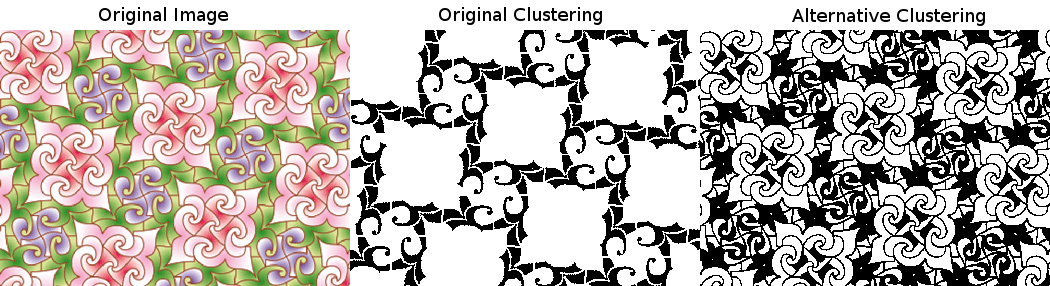
\includegraphics[scale=0.4]{./Figures/Etchers_result.png}
\caption{دسته‌بندی جایگزین برای یک پترن مخصوص}
\label{flowers}
\end{figure}

\subsubsection{بررسی زمان اجرا}
در این بخش، به بیان نتایج مقایسه‌ی الگوریتم 
\lr{ISM}
با سایر الگوریتم‌ها، از نظر زمان اجرا می‌پردازیم.

\begin{figure}[h!]
	\centering
	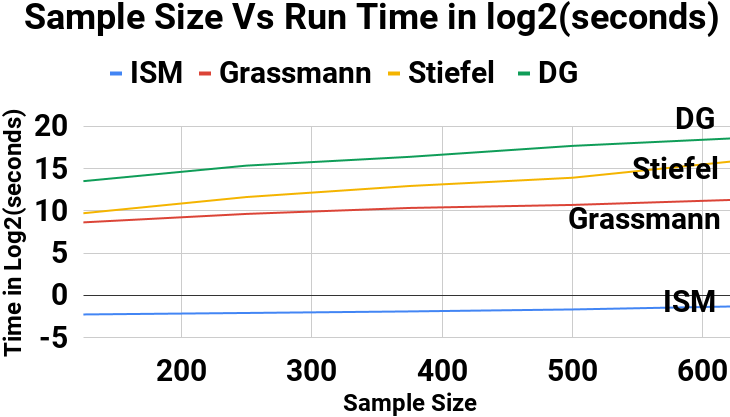
\includegraphics[scale = 0.35]{./Figures/runtime.png}
	\caption{زمان اجرای الگوریتم‌های مختلف بر جسب تعداد نمونه}
\end{figure}

مطابق انتظار، خم مربوط به الگوریتم 
\lr{ISM}
همواره پایین‌تر از منحنی سایر الگوریتم‌ها قرار دارد.


\chapter{پیشنهاد‌ها}

برای ادامه‌ی کار این مقاله، می‌توان چند پیشنهاد به صورت زیر داد:
\begin{enumerate}
	\item 
	مقاله‌ی حاضر، در محاسبه‌ی
	\lr{$W^*$}،
	به ارائه‌ی یک شرط کافی (معادله‌ی 
	\ref{final})
	برای احراز شرایط مرتبه‌ی دوم مسأله‌ی بهینه‌سازی بسنده کرده و شرایط مطرح‌ شده، لازم نیستند. بهتر بود اگر شرایط لازم برای برقراری شرایط مرتبه‌ی دوم مسأله‌ی بهینه‌سازی بررسی و مطرح می‌شدند. ممکن است این شرایط به الگوریتم دیگری برای محاسبه‌ی نقطه‌ی بهینه منتهی شوند.
	\item 
	در
	\cite{zhang2012kernel}،
	روشی برای محاسبه‌ی میزان وابستگی دو متغیّر تصادفی به شرط یک متغیّر تصادفی دیگر، بر مبنای متر 
	\lr{HSIC}
	بیان شده است. می‌توانیم از این روش استفاده کرده و مسأله‌ای مشابه مسأله‌ی این مقاله، در حوزه‌ی 
	\lr{transfer learning}
	مطرح کرد. مسئله به این صورت است که فرض کنیم داده‌های
	\lr{$X_1,Y_1$}
	 با توزیع
	\lr{$p_1(x,y)$}
	داریم. حال می‌خواهیم داده‌های
	\lr{$X_2,Y_2$}
	 با توزیع
	\lr{$p_2(x,y)$}
	را کاهش بعد دهیم و در این فرآیند از اطّلاعات موجود در داده‌های قبلی هم استفاده کنیم. مسأله می‌تواند به صورت زیر فرمول‌بندی شود:
	\[\max_{W} \;\HSIC(X_2W,Y_2|X_1,Y_1)\qquad \text{\lr{s.t. }} W^\top W = I\]
	به عنوان مثال، فرض کنید 
	\lr{$X_1$}
	داده‌های مربوط به خریدهای افراد مختلف از یک فروشگاه اینترنتی ایرانی باشد و 
	\lr{$Y_1$}
	سنّ این افراد باشد. همچنین فرض کنید که 
	\lr{$X_2$}
	اطّلاعات خریدهای افراد دیگری در یک فروشگاه اینترنتی غیرایرانی باشد و 
	\lr{$Y_2$}
	سنّ این افراد باشد. هدف آنست که با توجّه به داده‌های فروشگاه ایرانی و همچنین برچسب‌های داده‌ها، ماتریس
	\lr{$W$}ای
	بیابیم که داده‌ها را به نحو مناسبی کاهش بعد دهد.
	
\item 
استفاده از ایده‌های روش‌های عددی بهینه‌سازی غیرمحدب برای حل 
	\lr{IKDR}
   
   در بهینه‌‌سازی غیرمحدب، روش‌های زیادی برای فرار از بهینه‌های محلی معرفی شده‌اند. یکی از این روش‌ها، روش 
	\lr{Gradual Non-Convexity}
   است. در این روش، ابتدا تخمینی محدب از تابع هدف بهینه‌سازی زده می‌شود، سپس مسئله‌ی بهینه‌سازی برای این تابع هدف حل شده و جواب آن به دست می‌آید. سپس تخمینی دقیق‌تر (و غیرمحدب‌تر) ارائه می‌شود و الگوریتم بهینه‌سازی از نقطه‌ی نهایی الگوریتم قبل، شروع به حرکت در جهت کمینه می‌کند. این عملیات تکرار می‌شود و در هر مرحله مقداری عدم تحدب به مسئله افزوده شده و از نقطه‌ی پایان مرحله قبل برای شروع بهینه‌سازی استفاده می‌شود. روش‌هایی مبتنی بر 
	\lr{Gradual Non-Convexity}
      تا کنون برای حل دسته‌های وسیعی از مسائل کاربرد داشته‌اند، به طور مثال می‌توان به مسئله‌ی بازسازی تنک و کمینه کردن نرم صفر با قید‌ خطی اشاره کرد 
   \cite{SL0}.
   بررسی عملکرد الگوریتم‌‌های مبتنی بر 
	\lr{Gradual Non-Convexity}
      و سایر ایده‌های موجود در بهینه‌سازی غیرمحدب برای حل این مسئله نیز یکی از راه‌های پیش‌رو برای توسعه و بهبود روش‌های حل مسئله‌ی 
	\lr{IKDR}
      است.

\end{enumerate}


\lhead{}
%\begin{latin}
\bibliography{reference, long}

\bibliographystyle{ieeetr-fa}
%\end{latin}

%\begin{latin}
\begin{titlepage}
\vspace*{1cm}
\begin{center}


\includegraphics[width=4cm]{sharif.png}

 \large
Sharif University of Technology


Department of Electrical Engineering

\vspace*{1cm}
\large
\textbf{Final Report of Bachelor Project 1}

\vspace*{1.5cm}
\huge
\textbf{Blind Separation of Nonlinear Mixtures of Stochastic Processes} 
\vspace{1.5cm}

\Large

By:

\textbf{Behrad Moniri}
\vspace{1cm}

Supervisor:

\textbf{Prof.~Massoud Babaie-Zadeh}
\vfill
\large
\vspace{1.5cm}
Spring 2020
       

\end{center}
\end{titlepage}
\end{latin}

\پایان{نوشتار}
